\documentclass[a4paper,11pt,twoside,fleqn,openright]{memoir}
 
% Pakker
\usepackage[utf8]{inputenc} % Så må vi bruge æ, ø og å
%\usepackage[ansinew]{inputenc}
%\usepackage[danish]{babel} % Dansk opsætning
\usepackage[T1]{fontenc} % Hjælper med ordeling ved æ, ø og å. Sætter fontene til at være ps-fonte i stedet for bmp.
%\usepackage[scaled]{beramono} % Bedre monospace font
\usepackage{amsmath,amsfonts,amssymb} % God matematik
\usepackage{sistyle} % Enheder til fysik
\usepackage{array,booktabs} % Til gode tabeller
\usepackage{ragged2e} % For at kunnu lave tabeller med fast kolonnebredde, bruges sammen med 'array'
\usepackage{float} % Vi må nu bruge H som placering til floats
\usepackage{hhline} % Sum linie i tabel
\usepackage{multirow} % Fletning af rækker
\usepackage{multicol} % Fletning af kolonner
\usepackage{xcolor} % Vi kan bruge \color osv
\usepackage{colortbl} % Muligøre farver i tabeller
%\usepackage[danish=quotes]{csquotes} % Danske anførselstegn, brug enquote{}
\usepackage[english=british]{csquotes} 
\usepackage{graphicx} % Inkludere ekstern grafik
\usepackage[english,final]{varioref} % Vi kan anvende \vref
\usepackage{natbib} % Bedre litteratur henvisninger
\usepackage{pdfpages} % Inkludere en pdf side som en side  
\usepackage{acronym} % Smart akronymhåndtering
\usepackage{suffix} % Krævet af acronym
\usepackage{listings} % Til at inkludere kildekode direkte
\usepackage{lipsum} % Lorem ipsum dolar sit amet
\usepackage{caption} % Vi kan bruge \captionof
\usepackage{subfig} % Vi kan nu bruge \subfloat
\usepackage{calc} % Vi kan regne med tællere
\usepackage{changepage} % Vi kan ændre sidelayoutet lokalt
\usepackage{layout} % Vi kan se dimensionecne på vores layout med \layout
\usepackage[footnote,final,english,silent,nomargin]{fixme}
\usepackage[colorinlistoftodos]{todonotes}
\usepackage[pdftex,bookmarks=true,bookmarksnumbered=true]{hyperref} % Links i dokumentet
\usepackage{textcomp} % HVAD FANDEN GØR DENNE PAKKE?
\usepackage{threeparttable} % Så vi kan lave tablenotes (se latexbogen)
\usepackage{fixltx2e} % HVAD FANDEN GØR DENNE PAKKE?
\usepackage{minitoc} % Vi kan lave del inholdsfortegnelser forhåbentlig
\usepackage{color} % For use in the hilighting funcion

% For sjov pakker
\usepackage{marvosym}
\usepackage{wasysym}
%\usepackage{fourier}

\captionsetup{font={small,sf},labelfont=bf}

\pagestyle{companion}

% Litteraturliste stil
\bibliographystyle{plainnat}
%\bibliographystyle{abbrvnat}
%\bibliographystyle{unsrtnat}

% Andre egensakber for komandoer
\newcommand\Cpp{C\raisebox{\height / 2}[\height][\depth]{\tiny ++}} % Pænere C++
\newcommand{\mimg}[4]{\marginpar{\small \centering{\includegraphics[width=#1]{#2}\captionof{figure}{\newline #3}\label{#4}}}} % Margin billede
\newcommand{\lmimg}[4]{\marginpar{\small\centering{% Latex margin billede
  \def\svgwidth{#1}
  \graphicspath{{illustrations/}}
  \input{illustrations/#2.pdf_tex}
  \captionof{figure}{\newline #3}
  \label{#4}}}
}
\newcommand{\mnote}[1]{\marginpar{\small \textsf{\textbf{Note}\\{#1}}}} % Margin note
\newcommand{\mcd}[1]{\marginpar{\textsf{\textbf{\includegraphics[height=11pt]{formalities/media-optical}}\\\url{#1}}}} % CD-rom henvisning i margin
\newcommand{\cd}[1]{\includegraphics[height=9pt]{formalities/media-optical}\url{#1}} % CD-rom henvisning i tekst
\newcommand{\limg}[5]{\begin{figure}[#1]
  \centering
  \def\svgwidth{#2}
  \graphicspath{{illustrations/}}
  \input{illustrations/#3.pdf_tex}
  \caption{#4}
	\label{#5}
\end{figure}}
\newcommand{\head}[1]{{\slshape{#1}}\vspace{5mm}} % Header
\newcommand{\tail}{\vspace{3mm}\fancybreak{$*\quad*\quad*$}\vspace{3mm}} % Røvhul
\newcommand{\enhed}[1]{\hfill\hbox{[#1]}\qquad} % At indsatte heb enheder i firkantparentes i "equation"
\newcommand{\dB}[0]{\hbox{dB}} % At skrive dB oprejst
%\addto\captionsdanish{
%\renewcommand\appendixname{Appendiks}
%\renewcommand\contentsname{Indholdsfortegnelse}

% Make vectors bold instead of a arrow
\let\oldhat\hat
\renewcommand{\vec}[1]{\boldsymbol{#1}}
\renewcommand{\hat}[1]{\oldhat{\mathbf{#1}}}

\makechapterstyle{box}{
  \renewcommand*{\printchaptername}{}
  \renewcommand*{\chapnumfont}{\normalfont\sffamily\huge\bfseries}
  \renewcommand*{\printchapternum}{
    \flushleft
    \begin{tikzpicture}[line width=4pt]
      \draw (0,1) -- (0,0) -- (1,0);
      \draw (2,1) -- (2,2) -- (1,2);
      \draw[color=gray] (1cm,1cm) node { \chapnumfont\thechapter };
    \end{tikzpicture}
  }
  \renewcommand*{\chaptitlefont}{\normalfont\sffamily\Huge\bfseries}
  \renewcommand*{\printchaptertitle}[1]{\flushleft\chaptitlefont##1}
  \setlength\beforechapskip{-100pt}
}

\newif\ifchapternonum
\makechapterstyle{nickoe}{
\renewcommand\printchapternonum{\chapternonumtrue}
  \renewcommand*{\printchaptername}{} % Removes the 'Chapter' text
  \renewcommand*{\chapnumfont}{\fontfamily{pbk}\fontseries{m} \fontshape{n}\fontsize{80}{35}\selectfont } % Does some magic
  \renewcommand*{\printchapternum}{}
  %\hfill 
  %\fontfamily{pbk}\fontseries{m} \fontshape{n}\fontsize{80}{35}\selectfont % Makes a gigantic number
  %\chapnumfont\thechapter} % Removes the 'Chapter's number
  \renewcommand*{\printchaptertitle}[1]{%
  \noindent%
  \ifchapternonum%
  \begin{tabularx}{\textwidth}{X}%
  {\parbox[b]{\linewidth}{\raggedright \hskip -0.6em \chaptitlefont ##1}%
    \vphantom{\raisebox{0pt}{\chapnumfont 1}}}
  \end{tabularx}%
  \else

  \begin{tabularx}{\textwidth}{Xl}
  {\parbox[b]{\linewidth}{\raggedright \hskip -0.6em \chaptitlefont ##1} }
  & \raisebox{0pt}{\raggedleft \chapnumfont \hskip -0.5cm \thechapter \hskip -0.5cm}%
  \end{tabularx}%
  \fi
  \hrule
  }

  %\flushleft\chaptitlefont##1} % Prints the chaptertitle
  %\renewcommand{\afterchaptertitle}{\par\nobreak\medskip\hrule\vskip\afterchapskip}
  \setlength\beforechapskip{-100pt} % Makes the chapter go up on the page

}

\newenvironment{ffk}[0]% formel forklaring
{\begin{list}{}%
         {\setlength{\leftmargin}{\mathindent}}%
         \item[]%
}
{\end{list}}

% Akronyms formatering
\renewcommand*{\acsfont}[1]{#1}
\renewcommand*{\acffont}[1]{#1}
\renewcommand*{\acfsfont}[1]{#1}

% Farve definitioner
\definecolor{shadecolor}{gray}{.95}

\lstloadlanguages{C,VHDL,Java}
% Kodeformatering [C]
\lstnewenvironment{ccode}[2][]{
  \def\lstlistingname{Source code}
  \lstset{
    language=C,
    escapeinside={(*@}{@*)},  % a line can set with: (*@\label{c:labelname}@*)
    keywordstyle=\bfseries,
    commentstyle=\color{blue}, 
    basicstyle=\ttfamily\selectfont\footnotesize,
    numbers=left,
    numberstyle=\tiny,
    tabsize=2,
    showstringspaces=false,
    backgroundcolor=\color{shadecolor},
    frame=lines,
    captionpos=b,
    caption={#1},
    label={#2}
  }
}{}

% Kodeformatering [VHDL]
\lstnewenvironment{VHDL}[2][]{
  \def\lstlistingname{Source code}
  \lstset{
    language=VHDL,
    keywordstyle=\bfseries,
    commentstyle=\color{blue}, 
    basicstyle=\ttfamily\selectfont\small,
    numbers=left,
    numberstyle=\tiny,
    tabsize=2,
    showstringspaces=false,
    backgroundcolor=\color{shadecolor},
    frame=lines,
    captionpos=b,
    caption={#1},
    label={#2}
  }
}{}

% Kodeformatering [Assembler]
\lstnewenvironment{asmcode}[2][]{
  \def\lstlistingname{Source code}
  \lstset{
    language=[x86masm]Assembler,
    keywordstyle=\bfseries,
    commentstyle=\color{blue}, 
    basicstyle=\ttfamily\selectfont\small,
    numbers=left,
    numberstyle=\tiny,
    tabsize=2,
    showstringspaces=false,
    breaklines=true,
    backgroundcolor=\color{shadecolor},
    frame=lines,
    captionpos=b,
    caption={#1},
    label={#2}
  }
}{}

% Kodeformatering [Java]
\lstnewenvironment{javacode}[2][]{
  \def\lstlistingname{Source code}
  \lstset{
    language=Java,
    keywordstyle=\bfseries,
    commentstyle=\color{blue}, 
    basicstyle=\ttfamily\selectfont\small,
    numbers=left,
    numberstyle=\tiny,
    tabsize=2,
    showstringspaces=false,
    breaklines=true,
    backgroundcolor=\color{shadecolor},
    frame=lines,
    captionpos=b,
    caption={#1},
    label={#2}
  }
}{}

% Kodeformatering [XML]
\lstnewenvironment{xmlcode}[2][]{
  \def\lstlistingname{Source code}
  \lstset{
    language=XML,
    keywordstyle=\bfseries,
    commentstyle=\color{blue},
    basicstyle=\ttfamily\selectfont\small,
    numbers=left,
    numberstyle=\tiny,
    showstringspaces=false,
    backgroundcolor=\color{shadecolor},
    frame=lines,
    morekeywords={msgid, repeat, mmsi, navstat, rot, sog, posaccu, lon, lat, cog, truehead, timestamp, manoeuvre, raim, commstate, utc_year, utc_month, utc_day, utc_hour, utc_min, utc_sec, txbcast, name, aisver, imo, call, cargo, a, b, c, d, fixdev, eta_mon, eta_day, eta,hour, eta_min, draught, dest, dte, spare},
    captionpos=b,
    breaklines=true,
    caption={#1},
    label={#2}
  }
}{}

% \part omdefinering, nu med beskrivende tekst
\def\descpart#1#2{
  \par\newpage\clearpage % Page break 
  \vspace*{5cm} % Vertical shift 
  \refstepcounter{part}% Next part
  %\addcontentsline{toc}{part}{\texorpdfstring{\rlap{\thepart}\hspace{1.2em}#1}{\thepart\ #1}} % Adds entry to TOC 
  \addcontentsline{toc}{part}{\texorpdfstring{\rlap{\thepart}\hspace{2em}#1}{\thepart\ #1}} % Adds entry to TOC 
  {\centering \textbf{\Huge Part \thepart}\par}
  \vspace{1cm} % Vertical shift
  \thispagestyle{chapter} % Gives the pagestile an the memoir chapterpagestyle
  {\centering \textbf{\Huge #1}\par}
  \begin{center}
  {\parbox{9cm}{
  \vspace{2cm} % Vertical shift
  \noindent \slshape{#2} % Some text
  }}
  \end{center}
  \vfill\pagebreak % Fill the end of page and page break
}

%------------
\def\appendixpart#1#2{
  \par\newpage\clearpage % Page break 
  \vspace*{5cm} % Vertical shift 
  \addcontentsline{toc}{part}{\texorpdfstring{\rlap{\thepart}\hspace{2em}#1}{\thepart\ #1}} % Adds entry to TOC 
  \thispagestyle{chapter} % Gives the pagestile an the memoir chapterpagestyle
  {\centering \textbf{\Huge #1}\par}
  \begin{center}
  {\parbox{9cm}{
  \vspace{2cm} % Vertical shift
  \noindent \slshape{#2} % Some text
  }}
  \end{center}
  \vfill\pagebreak % Fill the end of page and page break
}


%------------

% At bruge figurer der fylder mere end brødteksten
% Der defineres nogle ekstra længder
\newlength{\fullwidth}
\setlength{\fullwidth}{\textwidth}
\addtolength{\fullwidth}{\marginparsep}
\addtolength{\fullwidth}{\marginparwidth}
\newlength{\fullmargin}
\setlength{\fullmargin}{\marginparwidth}
\addtolength{\fullmargin}{\marginparsep}
% For at bruge det, skal man f.eks. gøre således:
%\begin{figure}[h]
%\begin{adjustwidth*}{-\fullmargin}{}
%\includegraphics[width=\fullwidth]{./sti}
%\end{adjustwidth*}
%\caption{Beskrivelse her}
%\laber{fig:label}
%\end{figure}

% \degC for grader C
% \arcdeg for gradtegn
\renewcommand{\epsilon}{\varepsilon}
\newcommand{\MATLAB}{M{\footnotesize ATLAB}}
\parindent 8pt

% Orddeling
% Ord der deles forkert kan skrives her, men bindestreg ved stavelser og mellemrum mellem ordene
\hyphenation{ar-bejds-in-ten-si-ve an-grebs-vink-ler ind-gangs-im-pe-dans ro-ta-ti-ons-en-ko-der deres clock-fre-kvens sys-tem-et na-vi-gate} 

\usepackage{bytefield}

\hypersetup{
  pdftitle={AAUB\AA D},
  pdfsubject={1st semester Control and Automation, Aalborg University},
  pdfauthor={Rasmus Lundgaard Christensen, Nick Østergaard, Frederik Juul, Atilla, Tudor},
  pdfcreator=LaTeX,
  linkcolor=black,
  citecolor=black,
  filecolor=black,
  urlcolor=black
}

\begin{document}
\chapterstyle{nickoe}
\frontmatter
\author{Nick Østergaard \and Rasmus Lundgaard Christensen \and Frederik Juul \and Attila Fodor \and Todor Muresan}
\title{An autonomous marine environment surveying platform}
\date{\today}
\maketitle
\begin{center}
Worksheet \#42 by group 12gr730
\end{center}



\cleardoublepage
%\input{formalities/titlepage}
%\input{formalities/preface}
%\input{formalities/terminology}

%%%%%%% Maybe we should have an overview of the system here
\cleardoublepage
\tableofcontents


\mainmatter
\chapter{Introduction}
Measuring environmental parameters in and around the water in Greenland (or any coastal nation) is a time consuming task. Today measurements are carried out by manually navigating large vessels up and down along the coastline and into the fjords. 

An example where this could be highly efficient would be at the Fukushima accident 2011. As seen on figure \ref{img:fukushimaradiation} there exists no measurements of the radiation in the water, due to the danger and resource demand of sending a manned expedition. Only estimates of the radiation level in the water exist, and therefore it is impossible to say what effects the radiation have had on the surrounding maritime life, as well as what proximity margin should exist. A fleet of small autonomous vessels would be able to quickly give an overview of the damage caused, as well as the spread and strength of the radiation.
\mimg{0.3\textwidth}{img/fukushima.pdf}{At the site of the 2011 Fukushima accident only landside radiation measurements exist}{img:fukushimaradiation}
Another purpose of these measurements, which will be the primary focus for this project, could be to measure the water depth for bathymetric surveys \cite{StweartOceanography}. This would allow for safer voyages in and around the coastlines, and for general environmental studies. 

These measurements are today carried out by one large vessel, which could be exchanged for several smaller ones to reduce the surveying time and labor cost. This would make for a faster measurement of the coastline as well as giving an opportunity to measure previously un-surveyed waters due to costs. 

Reducing the size of a vessel, poses some other challenges in regards to the weather conditions and other environmental parameters, that has a much larger influence on small scale vessels, than on larger ones.
Limitations are also imposed from the availability of power for the boats,  the noise of measurements as well as limitations on the availability of computing power and communication links. This paper will deal with how such a surveying vessel can be developed, and still measure the water depth whilst under the influence of the above.

A challenge using a single beam transducer to measure water depth is the roll/pitch of the craft. Figure \vref{fig:beamer} illustrates this problem, where an induced pitch of the ship (eg. a wave) makes it impossible for the vessel to make a precise measurement.

\begin{figure}[h]
\centering
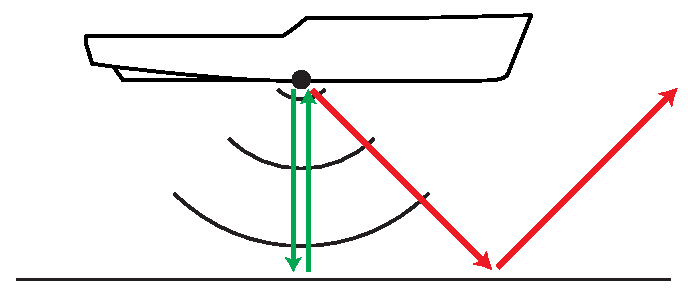
\includegraphics[width=0.5\textwidth]{img/beamer}
\caption{Overview of a depth mapping system. The green represents a measurement shot directly down and the red represents a measurement with induced pitch on the ship}
\label{fig:beamer}
\end{figure}

Another challenge, using a fleet of measurement boats, would be how to enable them all to coordinate and effectivize their effort. This could be done by having a mothership which would be in charge of coordinating and controlling the smaller ships. This larger ship would be able to store larger amount of energy, and be able to charge the smaller ships as needed. Due to this easy access to power it would be able to turn up signal strength and computing power as needed. This way it would be possible to reduce the requirements for the hardware aboard the ships, while still having sufficient hardware to compute complex algorithms necessary for control. Having this process centralized, however, offers some additional challenges. Packetloss and limited communicationspeed demand a robust system where these conditions are addressed. In this project the effect of packetloss and limited available data is analyzed and a solution based on an implementation of a kalman filter is suggested.

\chapter{Hardware considerations}

Because of the practical nature of the project, there are some things that have to be taken into account from a hardware point of view.

\section{LLI electronics}
The \ac{LLI} electronics is a plug and play device that controls several smaller ship instances. It provides outputs to control the actuators and motors as well as basic sensor readings to the \ac{HLI}.

The \ac{LLI} has been designed to allow for the above functionality. As described in section~\vref{sec:platform} the \ac{LLI} is an embedded platform, for which an Atmel AVR microcontroller has been chosen. The main control board is an Arduino Mega 2560, and a shield interface to all peripherals has been designed~\vref{chap:schema}.

The final LLI supports the following features:
\begin{description}
\item[Serial]\hfill \\ interface to the \ac{HLI} with a baud rate of 115200 bps
\item[PWM]\hfill \\ outputs for actuators
\item[I$^2$C]\hfill \\ option for aux communication
\item[Analog]\hfill \\ inputs for various sensors
\item[Relay driver]\hfill \\ output
\item[5V]\hfill \\ regulated output
\end{description}

More detailed information about hardware layout~\vref{fig:lli-hw} and the hardware schematic~\vref{chap:schema} can be found in the appendix.

\section{Lithium Polymer batteries}

	Lithium Polymer batteries have been chosen for powering the boat motors as well as for all the electronics, because they offer a very high specific energy and energy density, and can be charged in a relatively short period of time. 

\subsection{Energy calculations}
	
	Each battery is composed of 4 series connected cells with a nominal voltage of 3.7 V, making a total of 14.8 V. There will be 6 such batteries, each storing 3200 mAh worth of charge, which yields a total of $ 6 \cdot 14.8 \text{ V} \cdot 3.2\text{ Ah} = 284.16 \text{ Wh} $, around 1 MJ of energy.
	
	There are two separate electrical circuits: a power circuit for the motors for which there are 5 dedicated batteries connected in parallel and the electronics circuit which is separated in order to avoid noise in the digital circuitry. These two are alloted 236.8 Wh and 47.36 Wh respectively.
	
	\subsection{Battery care and charge meters}
	
	Due to the delicate nature of Li-Po batteries, it is absolutely required to never over-charge or over-discharge them because there is a high risk of permanent damage to the batteries. If the temperature continues to raise, there is even a risk of fire and/or explosion. In order to prevent this, we are using a dedicated Li-Po charger with an included balancer, which ensures that none of the cells in the batteries go above the absolute maximum of 4.2 V while charging.
	
	The problem of over-discharge is solved in the power circuit due to the fact that the brushless motor controller has a safety switch which does not allow any cell to drop below 3 V, which would cause permanent damage to the batteries, as they cannot recover after being over-discharged. 
	
	The electronic circuit can drain the batteries more than the maximum limit though. In order to prevent this from happening, we implemented a couple of battery level monitors that are integrated in the \ac{LLI} module and, which can compute the battery levels, thus allow the user to retrieve the boat in order to charge it. They should also include a master kill switch that can save the batteries as well.

\section{Electronics design}

	\subsection{Bow thruster controller}
	\label{subsec:bow thruster controller}
	
	The bow thruster controller is a circuit whose function is to provide power to the bow thruster, under the control of the \ac{LLI}. This uses a L298 H-bridge connected to a logic gate, so that it can be driven with just two signals: direction and \ac{PWM}.
	
	Another use of this circuit is to provide a lossless voltage level conversion from the batteries' nominal 14.8V to the motor's 7.2V rated voltage. That means that the maximum theoretical duty cycle of the PWM bow thruster control signal is $ 14.8 / 7.2 = 48 \% $. This, however, is not the actual value that will be used, due to the fall time of the L298 chip, which is pretty big at the 1kHz PWM frequency. By using an oscilloscope to measure the True RMS value of the electronic circuit's output, it was empirically determined that the maximum pulse width value is 33\%. 
	The motor used to drive the bow thruster also has a minimum starting voltage for which the PWM minimum duty cycle was empirically determined to be around 5\% in this case.
	
	Since the L298 chip has two H bridges inside it, the designed board which can be viewed in the appendix \vref{appendices:bow thruster schematic} includes the circuitry and parts for the two controllers, since it would provide redundancy in case one of them is overloaded or otherwise stops functioning.
	
\section{Motors and propellers}

The ship is equipped with two brushless Graupner Inline 750 14.8 V motors, each driving a horizontally mounted propeller. These are very powerful, as they are capable of working with 80 Amps of current. This makes the absolute maximum consumed power to be 1.1 kW per motor. Each of the motors are connected to a shaft and a brass propeller with a diameter of 5 cm.

\chapter{Platform}
\head{This chapter describes the platform to introduce a system overview. This helps to understand the physical interconnections that exists between modules.}

\noindent Ths total system consists of a wide range og modules, which are different components og sensors and actuators. Theese modules are connected to a \ac{LLI} and \ac{HLI} computing device. The \ac{LLI} is a micontroller, which takes vare of the basic functions of the platform, such as communicationg with basic sensors and actuators. The software for this is embedded and writen in C for avr-gcc compiler.

The \ac{HLI} is a x86 comnpatible computer of some sort that is able to run the higher abstraction layer code written in Python. This higher abstracion layer contains the onboard generation og waypoints of map data, to calculate the desired heading and speed for the vessel. This also calculates the stuff for the state space model which in turn talks to the \ac{LLI}.

Some modules that is connected to the \ac{LLI} is not handled by the \ac{LLI} itself, but forwards the data to the \ac{HLI} which uses this data for the control. A illustration of thsi can be seen on figure~\vref{fig:vessel-block-overview}.


\begin{figure}[htbp]
	\centering
	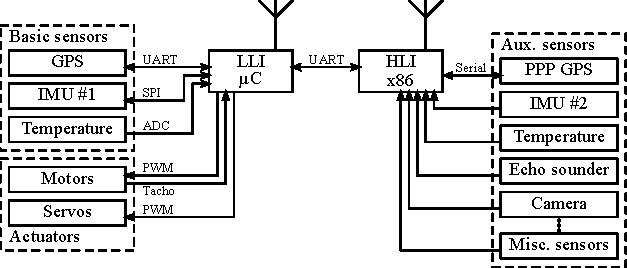
\includegraphics[width=\textwidth]{img/vessel-block-overview-electrical}
	\caption{Overview of electrical interconnections between \ac{LLI} and \ac{HLI} together with periphal modules.}
	\label{fig:vessel-block-overview-electrical}
\end{figure}

\chapter{Ship Design}
AAUSHIP1 has been designed by the ASV group during their 6th semester and is extensively designed in a 3D modeling program called RhinoCeros. The plan is to get the ship molded in plastic. As this process is expensive, it's quite important that we agree on the final design of the ship before we send it to the processing company. 

This ship is designed using a tool called Lofting, which takes some lines that runs along the ship, and then generates a surface from these. As none of us have any experience in creating ships - the design is loosely based on what we "think" is a good hull design. 

However, to further strengthen the structure, inlays are made by slicing a box at the edges of the ship hull. These are then to be produced in the machine workshop at the department of electronics. 

To get a better understanding of ship dynamics a rapid prototyping technique have been used, where 3D models of the ship have been printed - and if it didn't live up to our demands (visually deciding if the design was flawed), a revised model was then printed. Using an iterative process - the final design was reached.

\section{Bow thruster}
The ship design includes a bow thruster, which can be used to perform precision maneuvers in tight spaces. This component is not currently included in our control algorithms, because it has little or no effect on the ship when used at speeds above \todo{what speeds?}. It will be controlled by the \ac{LLI} with a direction and a \ac{PWM} signal. 

The electronic design of the bow thruster controller can be found in subsection \ref{subsec:bow thruster controller}: Bow thruster controller.

\section{Ship hull}

The hull of the ship follows a soft-chined displacement design, because in normal operating conditions the static buoyancy will dominate over dynamic. This shape affected less by the currents of the sea, and more by the wind. According to the data series of the British Oceanographic Data Centre\footnote[1]{https://www.bodc.ac.uk/data/online$\_$delivery/nodb/search/} near the shores of Greenland the drift caused by the steady currents is generally higher than the wind with a more randomly distributed blowing direction.

\begin{figure}[hullshape]
	\centering
	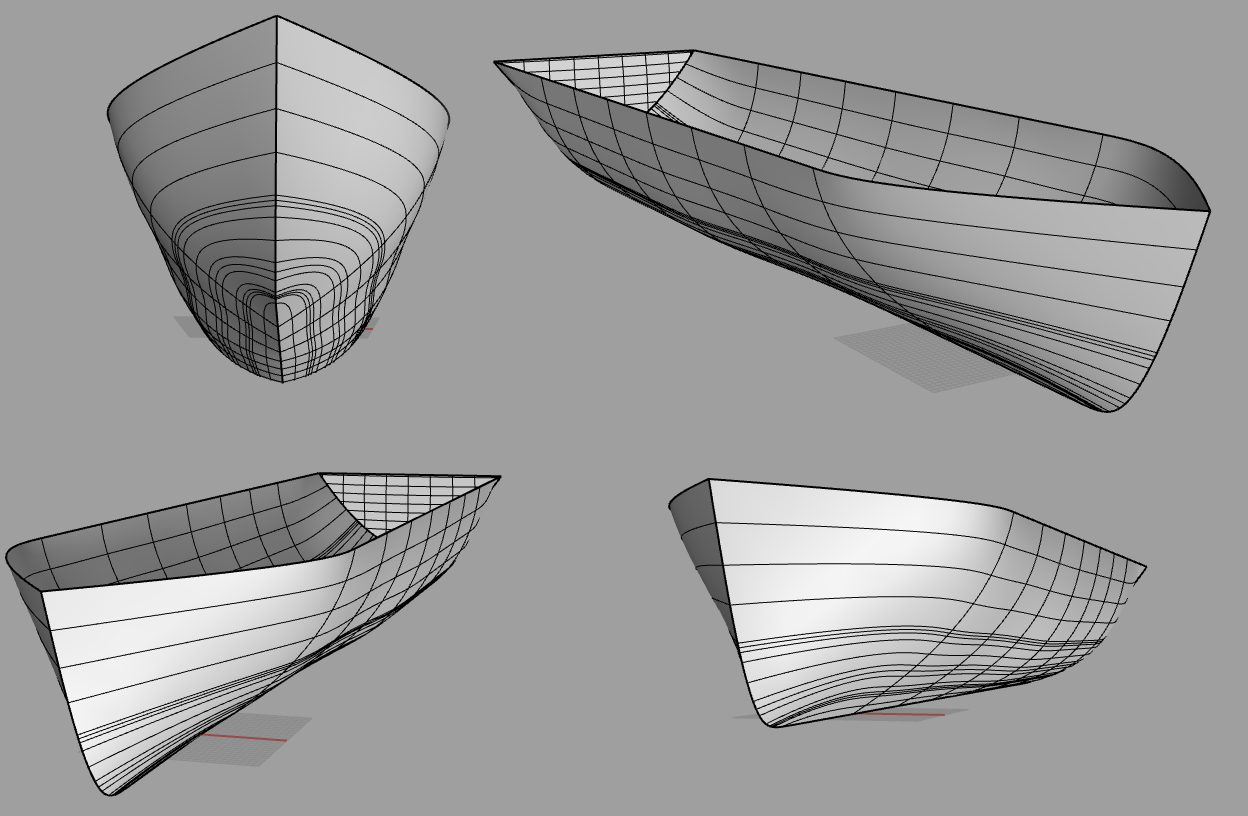
\includegraphics[width=\textwidth]{img/render/rendermontage.png}
	\caption{The shape of the hull}
	\label{fig:vessel-block-overview}
\end{figure}

The ship is outfitted with powerful main engines, so the vessel can perform fast and precise maneuvering without the bow thruster. Though these engines provide a lot of dynamic range, the ship hull was not designed for high speed \ref{jumping}. The problem is caused by the size and power of the propellers. At slower speeds the effect ceases \ref{jumping}.
Mirroring the setup and reversing the rotation movement would solve the pushing problem, but instead the back of the ship is pushed upwards, and air is sucked between the propellers. Instead, an additional vertical fin has been installed above the propellers, which keeps the water from being pushed upwards. As a positive side effect, the water after the hull is significantly less disturbed, thus the drag has been reduced as well. This has a positive effect on the range through the battery life \ref{fin}.

\begin{figure}[jumping]
	\centering
	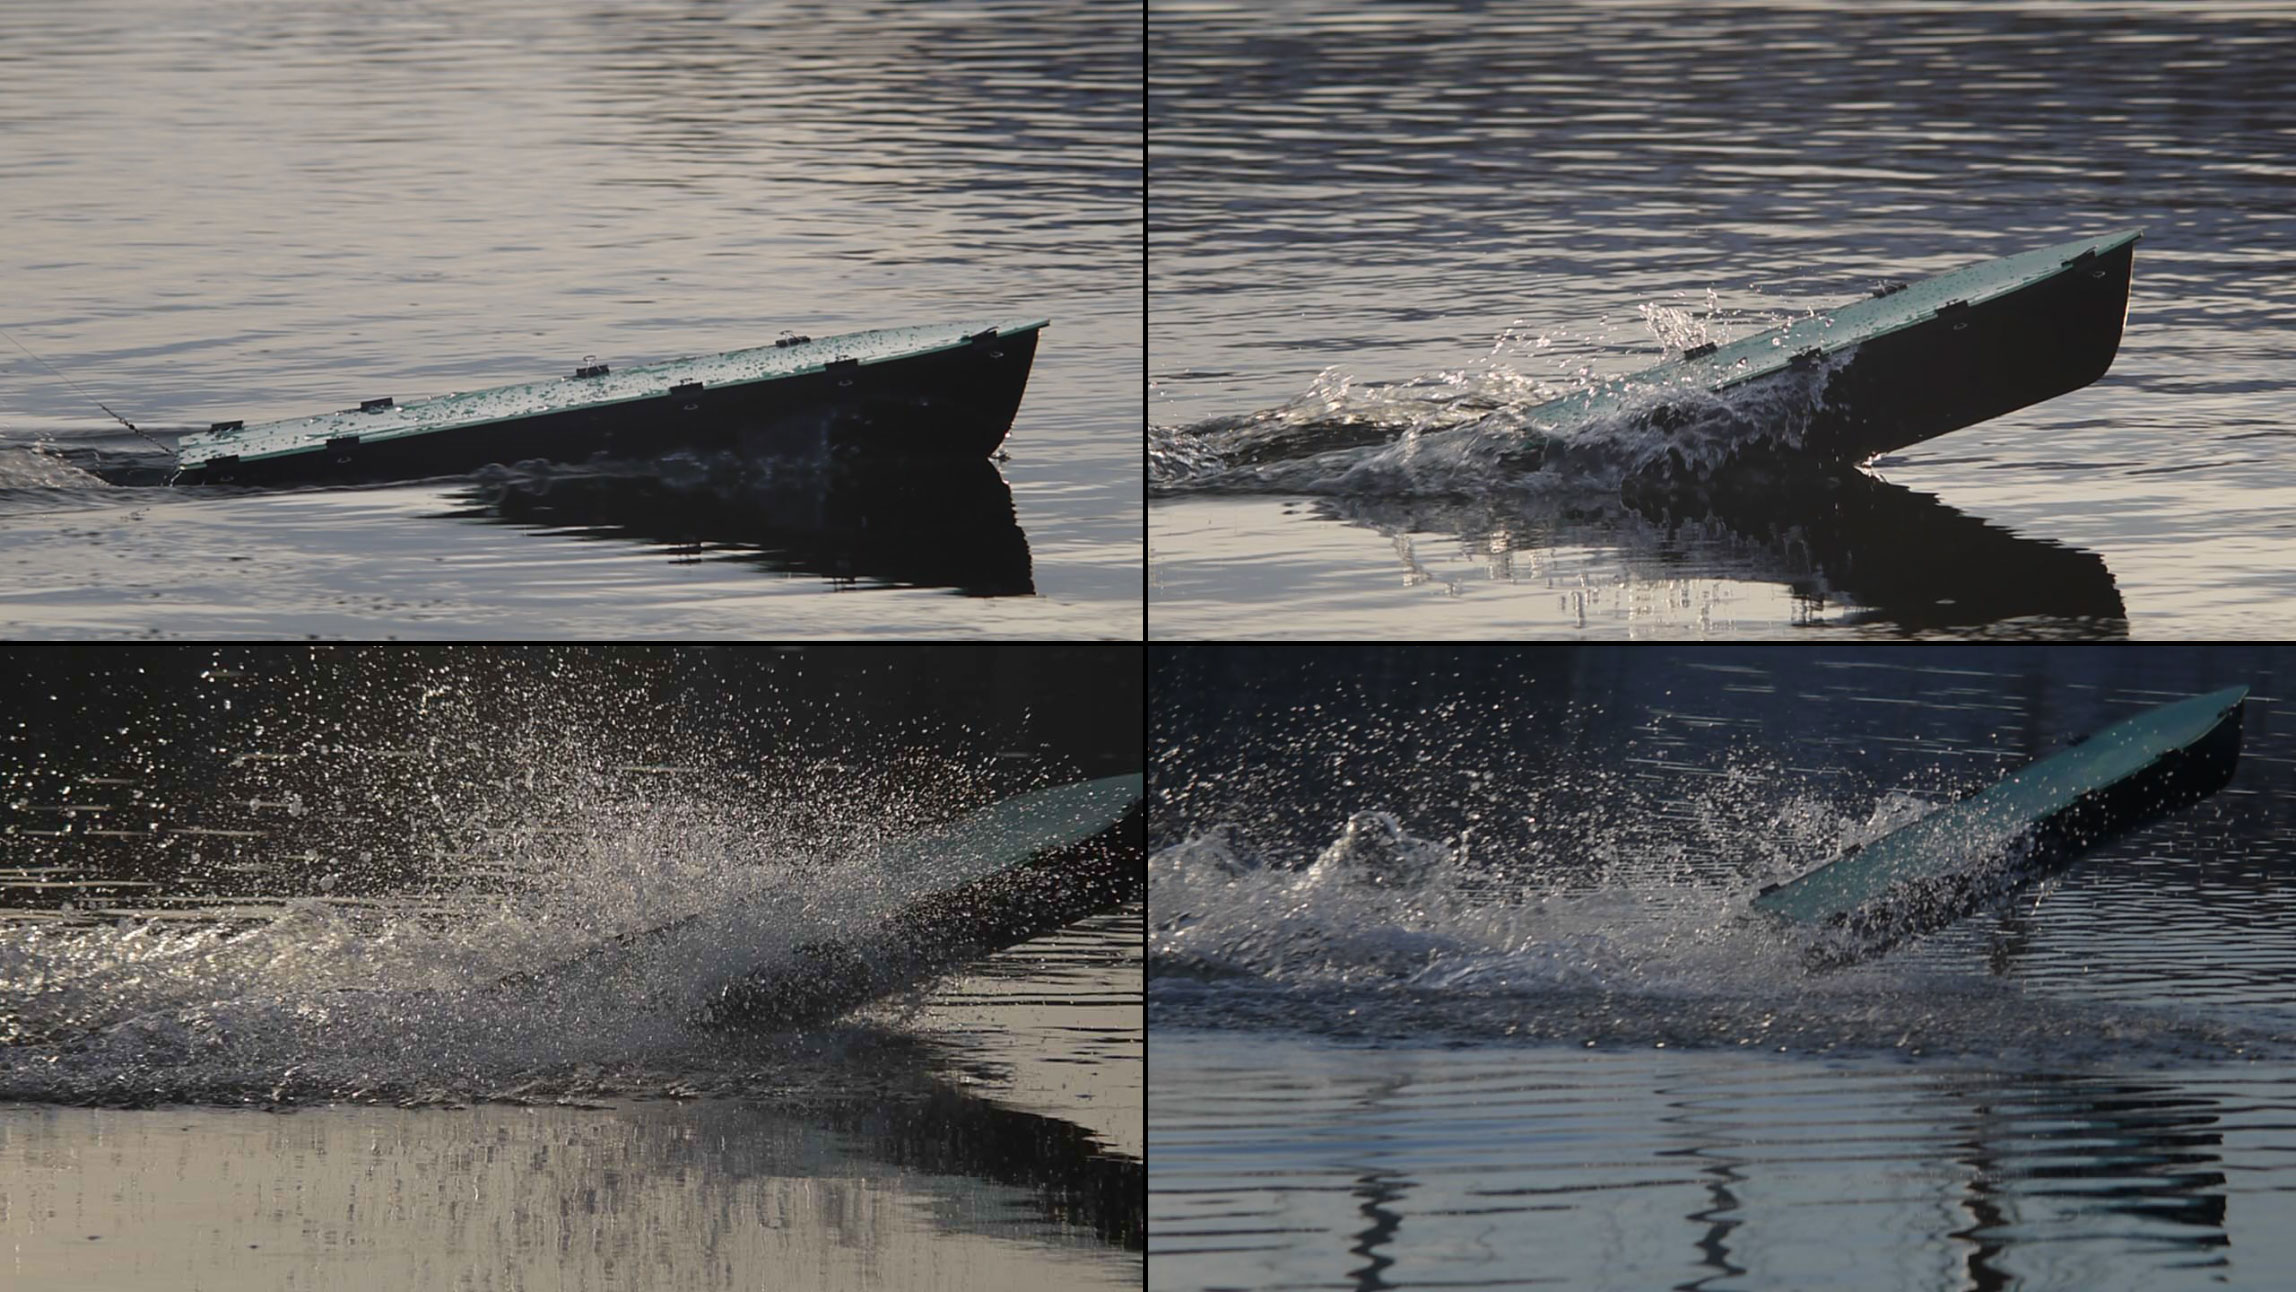
\includegraphics[width=\textwidth]{Pictures/VerticalJumpingTele.jpg}
	\caption{An excessive and unregulated bouncing can be experienced at high speeds.}
	\label{fig:vessel-block-overview}
\end{figure}

\begin{figure}[waterpushup]
	\centering
	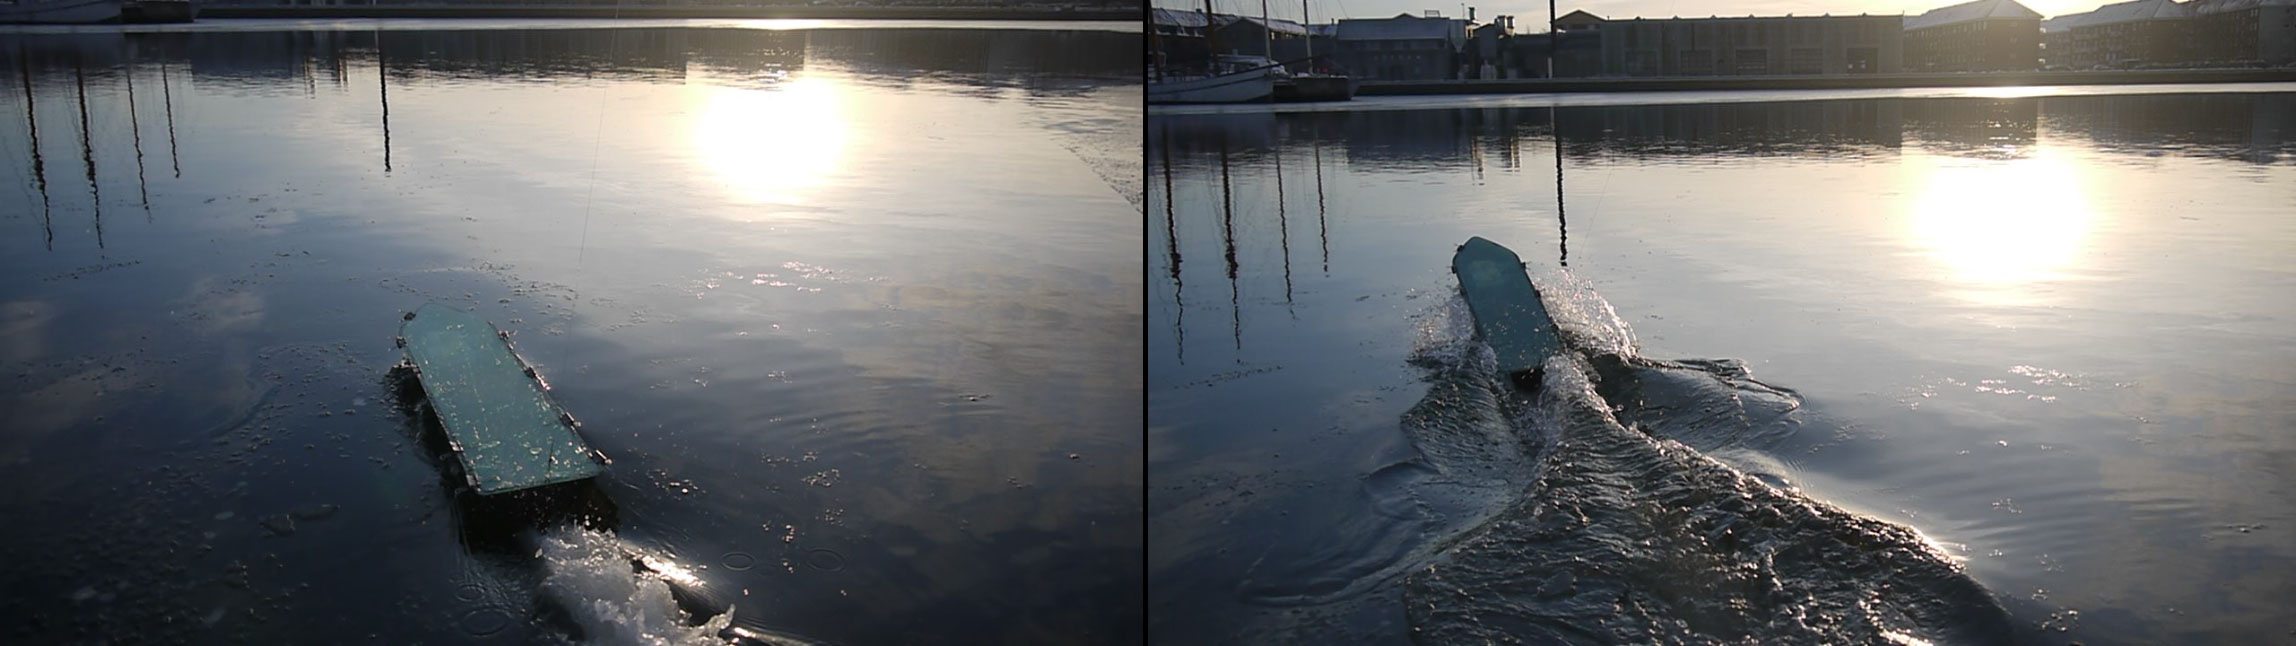
\includegraphics[width=\textwidth]{Pictures/forward.jpg}
	\caption{The power of the two engines force the water upwards between the propellers, therefore pushing the back of the ship down}
	\label{fig:vessel-block-overview}
\end{figure}

\begin{figure}[fin]
	\centering
	\includegraphics[width=\textwidth]{Pictures/Fin.jpg}
	\caption{The rotating propellers with the fin mounted above them. The engine power is set in the normal operation range}
	\label{fig:vessel-block-overview}
\end{figure}

\section{Parts list}
To develop the ship, a wide range of components had to be chosen. There are several things to be taken into consideration when designing a scale ship from scratch. The first component decided upon is the engines. As the ship should be able to cope with rather powerfull streams a powerfull propulsion system had to be chosen. The main propulsion unit consists of 2 Grapuner Brushless 750 14.8 V 1200W engines - which together produces around 3 HP at maximum input. With these powerfull engines we have a large dynamic range, that allows for fast acceleration and a fast maneuvering, as well as navigating in strong currents. 

The propellers are 2 counterrotating Raboesch brass propellers with a radius of 5 cm. 

For power, the ship is fitted with 6 4-celled Lithium-Polymer batteries, each holding up to 3.2 Ah. These will be divided into different sections, 4 serving the main engines, and 2 serving the onboard controls. If the batteries run at full power (draining a maximum of 80 Amps) the ship will be able to sail for 5 minutes, however, a scenario where the engine runs at full power with a brake on the propellers are unlikely.

Measurements show that the engines run at 60/60 (with a 500 max) they drain 2.5As combined, this will give an operation time of 5.1 hours - thus giving quite a big range on the ships. Assuming a 1 m/s velocity kept constantly for 2.5 hours, this gives a range of 9 kilometers forth and 9 kilometers back or being able to measure an area of 1 x 1 km in strips 100 meters apart and still have surplus power.
\chapter{FAPS LLI interface}
\label{chap:Protocol}
\head{Documentation for the \ac{LLI} part of the system. This describes the packet format and defines all commands.}
\section{Standard format of messages}
%To develop a suiting protocol for AAUSHIP1, the data to be sent via this is looked at in more detail in section~\vref{sec:lli-bandwith}. For instance, the \ac{IMU} has serveral different outputs, and receiving them all in one big stream might increase the load on the network, so splitting these up could free up some bandwidth which could be used for other (and more important) tasks. \todo{How can the last statement be true?}

To develop a suiting protocol for AAUSHIP1, the data to be sent via this is looked at in more detail in section ~\vref{sec:lli-bandwith}. For instance, the \ac{IMU} has several different outputs, which needs to be processed independent of each other. Because of this, they are broken into separate packages, each with their own ID and checksum. This simplifies parsing and allows the protocol to easily be expanded to other sensors and actuators which were not included in the original design. A short, single state packet limits the effect of a flipped bit, since only a single state has been lost, compared to a packet containing all information.

As both the \ac{IMU} and \ac{GPS} is sending packets of varying size, the data field in the protocol should be variable. However, there are some fixed elements, which is possible to decide now. The number of sensors/actuators connected to the \ac{LLI} can by design not be more than 256, which makes way for a 1-byte device resolution. As each device might contain several outputs (as seen from the \ac{IMU}) each device ID is then given an additional byte for message IDs. In addition to this header a length byte is contained to describe the length of the data field, to make it easier to parse. Lastly a \ac{CRC} checksum is added on the end to verify the content. Figure~\vref{fig:bytefield} depicts the packet structure. Everything other than the data field is fixed length as described in table~\vref{tab:general}. 
The data field can be either binary or ASCII, depending on the source. It is desired to limit the amount of calculations necessary at the LLI, seeing as the power of the HLI is many times greater, as well as the implementation being simpler.

\begin{figure}[h]
\centering
\begin{bytefield}{30}
\begin{rightwordgroup}{Header}
\raisebox{-1mm}{$\underbrace{\raisebox{1mm} {\bitbox{1}{\texttt{\$}}  \bitbox{5}{Length}   \bitbox{5}{DevID} \bitbox{5}{MsgID}}}_\mathrm{Header}$}%
\raisebox{-1mm}{$\underbrace{\raisebox{1mm} {\bitbox{16}{Data field }}}_\mathrm{Variable\ length}$}\bitbox{4}{CRC16} 
\end{bytefield}
\caption{Generic message bytefield}
\label{fig:bytefield}
\end{figure}

%The packet bytes are arranged as little endian (MSB first), and such should the numbering og bytes also be, i.e. the start start characther comes first when transmitted and ends with the end character which is the newline character.

The packet bytes are little endian (MSB first), which is consistent throughout the packet. The data field is arranged as always being a full number of bytes, to simplify transmission and receiving. This conforms to the RS232 standard.

\begin{table}[htbp],
	\centering
	\begin{tabular}{llll}
		\toprule
		\textbf{Field name} & \textbf{Size [bytes]} & \textbf{Type} & \textbf{Description}\\
		\midrule
		Startchar & 1 & uint8 & Start character (\texttt{\$}) \\
		Length & 1 & uint8 & Length of data field in the range 1--255\\
		DevID & 1 & uint8 & Device identifier \\
		MsgID & 1 & uint8 & Message identifier \\
		Data & 1--255 & uint8 & Data portion (binary or ASCII )\\
		Checksum & 2 & uint8 & CRC-16 checksum on data part \\

		\bottomrule
	\end{tabular}
	\caption{General description of the packet format}
	\label{tab:general}
\end{table}

The device ID (DevID) also serves as the priority of the packets, enabling more important packages to be sent prior to less important ones. For example; auxillaury parameters as temperature measurements are less important in time than navigational informations from the \ac{IMU} which has to be precisely known in time and preferably periodically.

\section{Message definitions}
%This is the list of all supported messages for the LLI interface. The messages is the interface to every thing that could be of interest for the HLI, i.e. sensor measurements and actuator control. The list of field descriptions in the following ommits the generic fields, with start character and checksum.
The initial list of supported devices and message IDs is given in table \ref{tab:commands}. The initial devices are distributed evenly with 10 IDs between each device to allow for other new devices to be implemented with with lower, higher priority, IDs. The general functions of the LLI are implemented with the highest available priority, since it has the deadman switch implemented but a very low amount of regular activity.
From the definition of the DevID and MsgID each packet can be identified as having to do with a given part of the system. This is the same throughout the system. For some parts of the system, such as the motors, it is not possible to see whether the packet is a set or a get command, from the initial data structure. To mediate this, a "Read thruster" command is implemented, and should be implemented for all future actuators or other devices which are not just passively feeding back data. This would be achieved by sending a "Read thruster" packet to the LLI from the HLI. The LLI will neglect the data part of this message, as it unnecessary to understand the intention of the package. It will then respond with the same MsgID and  DevID, but with the data is has read from the MotorSpeed register.
To facilitate the Plug and Play nature of the system, the first 3 available MsgIDs are defined to have a set meaning. These are given in table \ref{firstmsgids}.
\begin{table}[h]
\centering
\begin{tabular}{ll}
\toprule
\textbf{MsgID} & \textbf{Definition}\\
\midrule
0 & List available MsgIDs along with their functionality\\
1 & Set options for device\\
2 & Read options from device\\
\bottomrule
\label{firstmsgids}
\end{tabular}
\end{table}
If a packet with MsgID 0 is sent to a device, the device will respond with a list of all available MsgIDs, along with their definition. If a packet with MsgID 0 is sent to DevID 0, the General LLI, it will respond with a list of available devices. If these device definitions adhere to a strict protocol, it will be possible to automatically configure an LLI and HLI implementing this protocol. This protocol will not be defined in this project, but the feature will useful in checking and validating the configuration.

An x in the first column indicates that funcitonality is implemented on \ac{LLI}.

\begin{table}[h]
\centering
	\begin{tabular}{llrrl}
	\toprule
	& \textbf{Message Name} & \textbf{MsgID} & \textbf{Data Size} & \textbf{Contains}\\
	\midrule
	\multicolumn{5}{l}{\textbf{0: General LLI	}}\\
	\midrule
	& List available devices & 0 & Up to 255 & Return a message for every available device\\
	& Set options & 1 & Up to 255 & Option bytes\\
	& Read Options & 2 & Up to 255 & Option bytes\\
	& Deadman Switch & 3 & 1 & On or off signal for actuators \\
	& Status & 4 & Up to 255 & Statuses of sensors and actuators \\
	x& Ping & 5 & 0 & Empty \\
	x& Pong & 6 & 0 & Empty \\
	& ACK & 7 & 0 & Empty \\
	& NACK & 8 & 0 & Empty \\
	& Build Info & 9 & Up to 255 & Commit, target, date\\
	& Surge & 10 & 1 & Speed\\
	& Turn & 11 & 1 & Turning velocity\\
	\bottomrule
	\multicolumn{5}{l}{\textbf{10: Actuators}}\\
	\midrule
	& List available commands & 0 & Up to 255 & Return a message for every available MsgID\\
	& Set options & 1 & Up to 255 & Option bytes\\
	& Read Options & 2 & Up to 255 & Option bytes\\
	x& Set PWM actuator 1  & 3 & 2 & Engine 1, starboard side (default)\\
	& Read PWM actuator 1 & 4 & 2 & Engine 1, starboard side (default)\\
	x& Set PWM actuator 2 & 5 & 2 & Engine 2, port side\\
	& Read PWM actuator 2 & 6 & 2 & Engine 2, port side\\
	x& Set PWM actuator 3 & 7 & 2 & Engine 3 (auxiliary)\\
	& Read PWM actuator 3 & 8 & 2 & Engine 3 (auxiliary)\\ 
	x& Set PWM actuator 4 & 9 & 2 & Rudder\\
	& Read PWM actuator 4 & 10 & 2 & Rudder\\ 
	x& Set PWM actuator 5 & 11 & 2 & Auxiliary\\
	& Read PWM actuator 5 & 12 & 2 & Auxiliary\\ 
	& Set PWM output 1 & 13 & 2 & Bow thruster\\
	& Read PWM output 1 & 14 & 2 & Bow thruster\\ 
	& Set PWM output 2 & 15 & 2 & Auxiliary\\
	& Read PWM output 2 & 16 & 2 & Auxiliary\\ 
	& Set PWM output 3 & 17 & 2 & Auxiliary\\
	& Read PWM output 3 & 18 & 2 & Auxiliary\\ 
	\midrule
	\label{tab:commands}
	\end{tabular}
\end{table}
\newpage

\begin{table}[h]
\centering
	\begin{tabular}{llrrl}
	\toprule
	\multicolumn{5}{l}{\textbf{20: IMU}}\\
	\midrule
	& List available commands & 0 & Up to 255 & Return a message for every available MsgID\\
	& Set options & 1 & Up to 255 & Option bytes\\
	& Read Options & 2 & Up to 255 & Option bytes\\
	& X-Acceleration & 3 & 2 & Acceleration in X-direction\\
	& Y-Acceleration & 4 & 2 & Acceleration in Y-direction\\
	& Z-Acceleration & 5 & 2 & Acceleration in Z-direction\\
	& X-Gyro & 6 & 2 & Gyroscope in X-direction\\
	& Y-Gyro & 7 & 2 & Gyroscope in Y-direction\\
	& Z-Gyro & 8 & 2 & Gyroscope in Z-direction\\
	& X-Mag & 9 & 2 & Magnetometer in X-direction\\
	& Y-Mag & 10 & 2 & Magnetometer in Y-direction\\
	& Z-Mag & 11 & 2 & Magnetometer in Z-direction\\
	& Temp & 12 & 2 & Temperature in IMU\\
	x& Burst read & 13 & 24 & Reading with all sensor data\\
	\midrule
	\label{tab:commands}
	\end{tabular}
\end{table}
\newpage
\begin{table}[h!]
\centering
	\begin{tabular}{lllll}
	\toprule
	& \textbf{Message Name} & \textbf{MsgID} & \textbf{Data Size} & \textbf{Contains}\\
	\midrule
	\multicolumn{5}{l}{\textbf{30: GPS}}\\
	\midrule
	& List available commands & 0 & Up to 255 & Return a message for every available MsgID\\
	& Set options & 1 & Up to 255 & Option bytes\\
	& Read Options & 2 & Up to 255 & Option bytes\\
	& Velocity & 3 & 2 & Velocity\\
	& Latitude & 4 & 4 & Latitude\\
	& Longitude & 5 & 4 & Longitude\\
	& Lat, Lon, Vel & 6 & 42 & Condensed RMC i.e. \texttt{122935.000,A,5700.8349,N,00959.1367,E,0.62}\\
	\midrule
	\multicolumn{5}{l}{\textbf{40: Temperature}}\\
	\midrule
	& List available commands & 0 & Up to 255 & Return a message for every available MsgID\\
	& Set options & 1 & Up to 255 & Option bytes\\
	& Read Options & 2 & Up to 255 & Option bytes\\
	& Temp 0 & 3 & 2 & Temperature \\
	& Temp 1 & 4 & 2 & Temperature \\
	& Temp 2 & 5 & 2 & Temperature \\
	\midrule
	\multicolumn{5}{l}{\textbf{50: Voltage}}\\
	\midrule
	& List available commands & 0 & Up to 255 & Return a message for every available MsgID\\
	& Set options & 1 & Up to 255 & Option bytes\\
	& Read Options & 2 & Up to 255 & Option bytes\\
	& Voltage & 3 & Up to 255 & Voltage\\
	\bottomrule
	\end{tabular}
\end{table}

The protocol is implemented as a class on the HLI


\section{General messages}

\begin{table}[h]
	\centering
	\begin{tabular}{llll}
		\toprule
		\textbf{Message name}  & \textbf{msgid} & \textbf{data size} & \textbf{Action}\\
		\midrule
		Deadman switch & 0 & 1 & Turn on or off actuators and wait for manual control \\
		Status of system & 1 & Up to 255 & Statuses of sensors and actuators \\
		Ping & 2 & Empty \\
		Pong & 3& Empty \\
		ACK & 4 & Empty\\
		NACK & 5 & Empty\\
		Build info & 6 & Up to 255 & Commit, target, date\\
		Surge & 7 & 1 & Speed\\
		Turn & 8 & 1 &\\
		\bottomrule
	\end{tabular}
	\caption{Byte field description of general messages (devid 0)}
	\label{tab:ack}
\end{table}

\todo{Expand each message row with rows of data fields}

\section{Actuator messages}
\begin{table}[h]
	\centering
	\begin{tabular}{llll}
		\toprule
		\textbf{Message name}  & \textbf{msgid} & \textbf{data size} & \textbf{Action}\\
		\midrule
		Actuators ON/OFF & 0 & 1 & Bit mask representing which actuators should be of and on\\
		Set right thruster & 1 & 2 & Speed (main thruster of only one) \\
		Set left thruster & 2 & 2 & Speed \\
		Set bow thruster & 3 & 2 & Speed \\
		\bottomrule
	\end{tabular}
	\caption{Byte field description of actuator messages (devid 1)}
	\label{tab:ack}
\end{table}

\section{Sensor messages}
\begin{table}[h]
	\centering
	\begin{tabular}{llll}
		\toprule
		\textbf{Message name}  & \textbf{msgid} & \textbf{data size} & \textbf{Action}\\
		\midrule
		Acclerometer & 0 & 1 & \\
		Gyrometer & 1 & 2 & \\
		Magnetometer & 2 & 2 &  \\
		GPS & 3 & 2 & GPGGA data \\
		\bottomrule
	\end{tabular}
	\caption{Byte field description of sensor messages (devid 3)}
	\label{tab:ack}
\end{table}




STATUS
gps
vsupply
under\_way
actuators\_on
autopilot\_on
cpu\_usage

ACTUATORS\_OFF

ACTUATORS\_ON

MARK\_HOME

GET\_POSITION

REPORT\_POSITION


\section{Analysis of data and bandwidth}
\label{sec:lli-bandwith}
To be able to evaluate if there is enough bandwidth on between the serial connections from LLI, HLI and ground station, an analysis is hereby conducted.


\todo{Remember 115200 baud, with 8N1, which mean that 80\% is the of that is the bit per secon}

\chapter{Packet Loss}
\label{chap:PacketLoss}

One of the features of the Kalman-filter is that it makes it possible to have a better reaction to a missing packet. This comes from the fact that a missing packet can merely be treated as a packet with very high noise, meaning a Kalmangain of 0. With a Kalmangain of 0, the measurement included in the packet will not be included in the next prediction. This is a key feature of the filter as well as a key feature of the project.
If a GPS measurement is lost the ship is effectively sailing blind. If however measurements of other parameters are available, it is possible to very effectively predict where the ship is positioned and which heading it has. With this information it is possible to still control the ship, remotely, until a new fix is received. This makes the system very robust in regards to packetloss, as it is estimated that only a limited amount of the packets will be lost. 

If we assume that 10$\%$ of the packets will be lost, regardless of the type, we can estimate the approximate average sampling rate. This can be calculated from equation (\ref{eq:packetloss}). This is quickly observable by the fact that a packetloss of 0 results the actual sampling rate, a packetloss of 50$\%$ results in half the sampling rate, and a packetloss of 100$\%$ results in an 0 sampling rate.
\begin{equation}
\hat{f_s} = f_s(1-p)
\end{equation}
\label{eq:packetloss}
\begin{tabbing}
Where \= $\hat{f_s}$ is the effective average sampling speed\\
\> $f_s$ is the actual sampling speed\\
\> $p$ is the probability for packet loss
\end{tabbing}
From this it can be seen that a system implementing this form of kalman filtering as a way to deal with packetloss can effectively be estimated as a lossless system with a lower sampling rate.
It can also be seen that there are two ways to generate a better estimate - reduce the probability of packetloss or increase the sampling rate.
If we assume a fixed samplingrate we can estimate $p$ and, in many cases, decrease it by increasing the signal strength. The increase in effective sampling rate is ofcourse dependent on the current value of $p$, as the gains from this is obviously non-linear. As seen in \todo{ref chapter with considerations about worse estimates during turning} the estimates become worse when the ship is turning. This can be mediated by turning up the signal strength to reduce the probability of packet loss, and therefore increasing the effective average sampling rate. 
\chapter{Control}
\label{chap:control}

\section{Overview of the control system}
This is an overview of the information flow for control in regard to the rest of the system containing, sensors, \ac{LLI} and \ac{HLI}.

\begin{figure}[htbp]
	\centering
	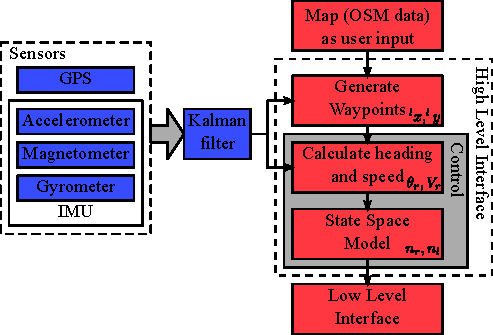
\includegraphics[width=\textwidth]{img/vessel-block-overview}
	\caption{Overview of control information flow in regard to the subsystems. The blue part indicates information that is not fetched directly to the control part, it is electrically connected to the \ac{LLI} whilst being forwarded to the \ac{HLI}.}
	\label{fig:vessel-block-overview}
\end{figure}

\todo{Illustrate on figure~\vref{fig:vessel-block-overview} where RF comms is or maybe that should be on the block overvieww diagram without regard to contorl abstraction}



In the First Stage the required heading of the ship is calculated that keeps the course closest to the planned waypoint.

In order to efficiently and accurately navigate along the path, a set of Sub-Waypoints is calculated for each route between two Waypoints. The main control strategy of the first path is to navigate through all of these SWPs in a predefined order, one by one. (Navigation Figure) The heading of the ship is defined in NED coordinate system. The required heading is determined by the law of Cosines, based on the Position of the Ship and the Position of the next Sub-Waypoint.
\begin{center}

\includegraphics[scale = 0.4]{img/ControlStrategyFigures/Law_of_Cosines.png}
\end{center}
Problems rise and corrections are necessary, if the heading of the ship $\theta$ is $\theta < -\pi$ or $\theta < \pi$. The heading of the ship is calculated based on the Gyro sensor and the heading can have any value in the form of: $$\theta = [-{\pi} ; \pi ] \pm 2*k*\pi$$. Before invoking the control procedure, all of the heading angles must be transformed into the $[-\pi ; \pi]$ interval.
This procedure causes a possible error though.

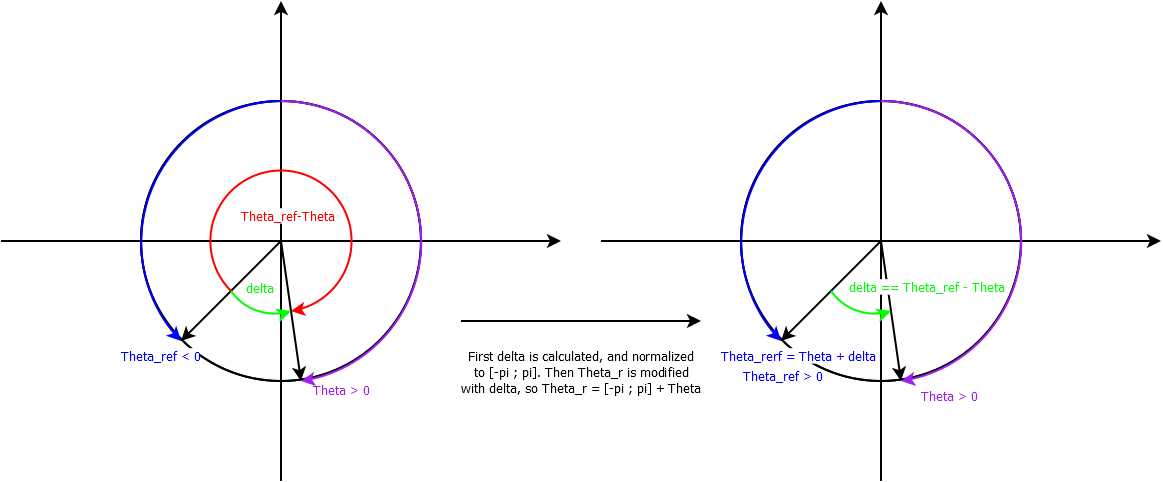
\includegraphics[width=\textwidth]{img/ControlStrategyFigures/Headings.png}

The required heading or the heading of the ship must be transformed into a different representation, where $$|\theta_{r}-\theta| < \pi$$. To keep a consistent heading representation, first the deviation angle $$\theta = \pi_{r}-\pi$$ is calculated, than transformed to the $[-\pi;\pi]$ interval and finally, with $\delta$ we can transform $\theta_{r}$ to $$\theta_{r}(\theta) = \theta + \delta$$.
If the conditions above are met, $\theta$ and $\theta_r(\theta)$ will always yield values that result in correct controller output.

\subsection{Subwaypoint Validity}

The overall navigation can be improved, if the Target SWPs are considered ''reached´´ in a certain distance. Optimally this distance (Validity distance) should be somewhat longer than the minimum turning radius of the ship ($R_{min}$). If it is shorter, the ship might not be able to reach the SWP, if it is way longer, the ship will divert from its course in turns.

%1. what is it
\todo{description}

%2. why are we using it


The reason for which the State Space representation was chosen is because it is a very simple, yet powerful way of modeling linear systems, allowing us to adjust and manipulate its dynamics in a very wide range of situations. 

%3. what are we using from it

\subsection{Linearizing the outputs}

Using Newton's second law of motion for forward  and rotational movement (F = m * A; T = I * W'), we can easily see that the inputs to our system will be F and T representing the forward force and the torque produced by the motors. It is worth mentioning that, since there are two propellers rotating in opposite directions, a torque that would induce a rotation around Z axis passing through the boat's center of mass only if the two propellers are rotating at different speeds.

These two rotational speeds N1 and N2 were initially included in the state space model as inputs to the system, as they could be controlled directly via a PWM pulse. This though proved to complicate matters because the relationship between the speeds of the propellers N1 and N2 and the force F and torque T generating accelerations is not a linear one. Because of this, our system would not be linear and would be beyond the scope of this project. 

\todo{insert formulas for [F, T] -> [n1, n2] transformation here}

In order to prevent this from happening, the state space model was updated to only calculate the force T and torque T necessary for driving and turning the ship, and this would keep our system linear. in order to transform from [T, F] to [N1, N2], another module was introduced in the system which would implement this non-linear function. 

This is a better solution anyway because if the state space model only outputs T and F, then it could be used for some other ship configurations, without modifications to the model, only to the module that translates the force and torque to N1 and N2. This, for example, can allow us to change the size of the propellers or their positions.

\subsection{Linearizing the drag forces}
\label{sect:Linearizing drag forces}

The drag forces acting on the bow of the ship while it's moving through the water are influenced by the area of the hull that is below water depth in the direction of movement, the density of the water, a drag constant $ C_{D} $ , and the square of the ship's speed components $ v_{x} $ and $ v_{y} $. 

A worthy note is the fact that the drag coefficient $ C_{D} $ will have two values depending on the direction of the ship's movement. When moving forward in the x direction, the coefficient $ C_{D}x $ will be approximated for a triangular shape, which is the closest simple shape that we have values for. For lateral movement in the y direction, $ C_{D}y $is given for a square box. These approximations should not present a problem in the operation of our control system as the errors ca easily be corrected and adjusted for by a good controller.

\[ D_{x}(v_{x}) = \frac{C_{Dx}\cdot\rho_{water}\cdot A_{front}\cdot v_{x}^{2}}{2} \]
\[ D_{y}(v_{y}) = \frac{C_{Dy}\cdot\rho_{water}\cdot A_{side}\cdot  v_{y}^{2}}{2} \]

Where $ D_{x}(v_{x}) $ and $ D_{y}(v_{y})$ are the drag forces dependent on the forward and lateral speeds respectively, $ \rho_{water} $ is the density of the water, $ A_{front} $ is the frontal area of the hull and $ A_{side} $ is the lateral area. 

The drag torque that is produced by the drag force acting on the hull of the ship, as the ship rotates through the water is dependent on the square of the angular velocity $ \omega $:

\[ \tau(\omega) = \frac{C_{D} \cdot \rho_{water} \cdot d \cdot (r_{f}^{4} + r_{b}^{4}) \cdot \omega^{2}}{8} \]

Where $ \tau(\omega) $ is the torque generated by the angular speed $ \omega $, $ d  $ is the depth of the ship that is submerged in water, $ r_{f} $ and $ r_{b} $ are the radii of the ship from the center of mass towards the front and back end, respectively.

These forces are obviously non-linear and thus cannot be integrated into the linear Kalman filter or State Space Model. Because we will usually use a constant speed it is feasible to linearize these forces for that value and not have big errors. The angular drag torque can also be linearized around a mean turning speed because the radii of the corners of the paths are also constant.

Approximation of the drag forces around the points of interest $v_{l} $ and $\omega_{l}$ is done using the first order term of the Taylor expansion:

\[ y_{l}(x) = f(a) + f'(a)(x-a) \]

Where $y = f(x)$ is the function we want to linearize around a value of interest $a$. Applying this formula to our situation yields:

\[ Dx_{l}(v_{x}) = \frac{C_{D}x\cdot\rho_{water}\cdot A_{front}\cdot v_{l}^{2}}{2} + (C_{D}x\cdot\rho_{water}\cdot A_{front})\cdot (v_{x}-v_{l}) \]

\[ Dy_{l}(v_{y}) = \frac{C_{Dy}\cdot\rho_{water}\cdot A_{side}\cdot v_{l}^{2}}{2} + (C_{D}y\cdot\rho_{water}\cdot A_{side})\cdot (v_{y}-v_{l}) \]

\[ \tau_{l}(\omega) = \frac{C_{D}y \cdot \rho_{water} \cdot d \cdot (r_{f}^{4} + r_{b}^{4}) \cdot \omega_{l}^{2}}{8} + \frac{C_{D}y \cdot \rho_{water} \cdot d \cdot (r_{f}^{4} + r_{b}^{4}) \cdot \omega_{l}}{4} \cdot (\omega - \omega_{l}) \] 

\begin{figure}[htbp]
	\centering
	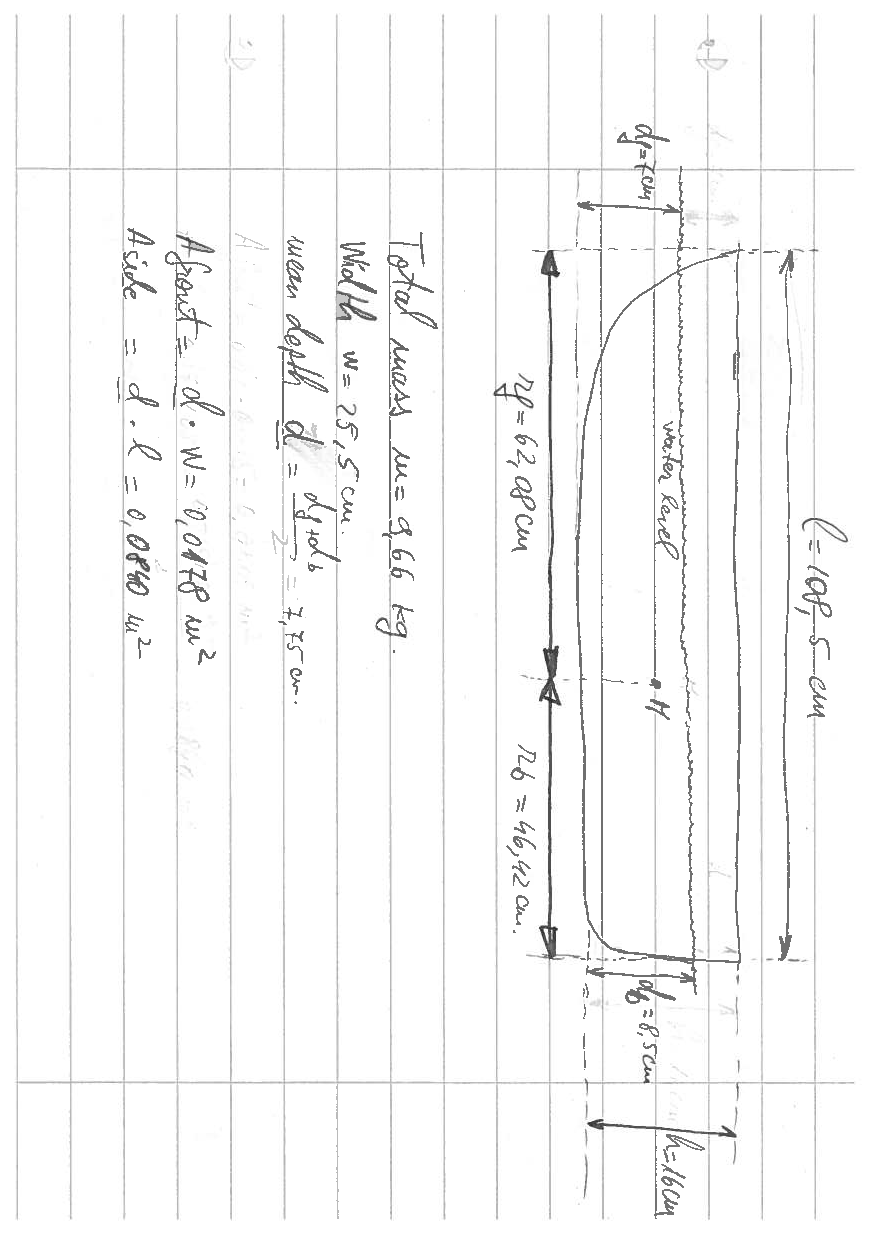
\includegraphics[width=\textwidth, trim=1.8cm 0cm 0cm 2cm, clip = true, angle = 90, width=\textwidth]{img/ship_sizes}
	\caption{Sketch of ship sizes as measured after the maiden voyage}
	\label{fig:ship_sizes}
\end{figure}

Given \vref{fig:ship_sizes}
 $ v_{l} = 1m/s $ ,
 $ \omega_{l} = 1 s ^{-1} $ ,
 $ C_{D}x = 0.5 $ (triangle) ,
 $ C_{D}y = 1 $ (box) ,
 $ \rho = 1000 kg/m ^{2} $,
 $ A_{front} = 0.0178 m^{2} $,
 $ A_{side} = 0.0840 m ^{2} $,
 $ d = 0.0775 m $,
 $ r_{f} = 0.6208 m $,
 $ r_{b} = 0.4642 m $,
the linearized formulas for the drag forces can be computed to be:


\begin{align}
 Dx_{l}(v) &= -4.45 + 8.9 \cdot v_{x} \\
 Dy_{l}(v) &= -42 + 84 \cdot v_{y} \\
 \tau_{l}(\omega) &= -1.88 + 3.77 \cdot \omega
\end{align}

From which we can identify the coefficients that correspond tot the linear relation $ y_{l}(x) = \alpha + \beta \cdot x $:\\
\begin{minipage}{0.3\linewidth}
\[ \alpha_{x} = -4.45 \] 
\[ \beta_{x} = 8.9 \]
\end{minipage}
\begin{minipage}{0.3\linewidth}
\[ \alpha_{y} = -42 \] 
\[ \beta_{y} = 84 \]
\end{minipage}
\begin{minipage}{0.3\linewidth}
\[ \alpha_{\omega} = -1.88 \]
\[ \beta_{\omega} = 3.77 \]
\end{minipage}


\subsection{Choosing the right states}

The variables we chose to be the states in our model are the speed of the ship in the forward direction in the ship frame $v$, the angular position of the ship's x axis relative to true North $\theta$ and the angular speed $\omega$.\\
\[\begin{cases}
F - F_{D} = m \cdot \dot{v}\\
T - T_{D} = I \cdot \dot{\omega}\\
\end{cases}\]

Where $ F $ and $ T $ are the force and torque produced by the propellers, $ F_{D} $ and $ T_{D} $ are the force and torque caused by water drag, $ m $ is the mass of the ship, $ I $ is the moment of inertia, $ \dot{v} $  and $ \dot{\omega} $ are forward and angular acceleration respectively.

The linearized drag force and torque from \ref{sect:Linearizing drag forces} can be substituted in these equations:
\begin{align}
 \dot{v} &= - \frac{\beta_{x} \cdot v}{m} + \frac{F}{m}\\
 \dot{\omega} &= - \frac{\beta_{y} \cdot \omega}{I} + \frac{T}{I}\\
 \dot{\theta} &= \omega
\end{align}

Note that we have also dropped the $ \alpha $ term of the equations because we're currently only interested in the dynamic behavior of the system. The $ \alpha $ offset will be compensated for when removing the steady state error. Consequently, these relations can be rewritten in a matrix notation as follows:
\[
\dot{
	\begin{bmatrix}
	 v\\
	 \theta\\
	 \omega
	\end{bmatrix}
}
=
\begin{bmatrix}
 -\frac{\beta_{x}}{m} & 0 & 0\\
 0 & 0 & 1\\
 0 & 0 & - \frac{\beta_{y}}{I}\\
\end{bmatrix}
\cdot
\begin{bmatrix}
v\\
\theta\\
\omega
\end{bmatrix}
+
\begin{bmatrix}
\frac{1}{m} & 0\\
0 & 0\\
0 & \frac{1}{I}\\
\end{bmatrix}
\cdot
\begin{bmatrix}
F\\
T
\end{bmatrix}
\]

This corresponds to the State Space Model equation:
\[\dot{X} = AX + BU\]

Since the output matrix we need is $ Y = \begin{bmatrix}v \\ \theta \end{bmatrix} $, the output equation
\[Y = CX + DU\]
becomes:
\[\begin{bmatrix}v \\ \theta \end{bmatrix}
 = 
\begin{bmatrix}
1 & 0\\
0 & 1\\
0 & 0
\end{bmatrix}
\cdot
\begin{bmatrix}
v\\
\theta\\
\omega
\end{bmatrix}
\]

So the system matrices are:
\[
A =\begin{bmatrix}
 -\frac{\beta_{x}}{m} & 0 & 0\\
 0 & 0 & 1\\
 0 & 0 & - \frac{\beta_{y}}{I}\\
\end{bmatrix}\\
B = \begin{bmatrix}
\frac{1}{m} & 0\\
0 & 0\\
0 & \frac{1}{I}\\
\end{bmatrix}\\
C = 
\begin{bmatrix}
1 & 0\\
0 & 1\\
0 & 0
\end{bmatrix}\\
D = 0
\]

\subsection{Discretizing for use with a particular timestep}

The system described so far is continuous and needs to be discretized before implementation in a computer algorithm, so we use the function c2d from MATLAB and the time step Ts in order to do this. \todo{explain more about c2d or what we will eventually use}

\subsection{Pole assignment}

For assigning poles, we use the lqr function implemented in MATLAB. This calculates the gain matrix $ F $ by minimizing the quadratic cost function:\todo{taken from here http://www.mathworks.se/help/control/ref/lqr.html}
\[
J(u)=\sum_{0}^{\inf} \{x^{T}Qx+u^{T}Ru+2x^{T}Nu\}
\]


\subsection{Reference gain}

A reference gain is calculated and implemented in order to counter the steady state error. This is calculated using the formula $ N = Nu+FNx $ \todo{insert refference to feedback book, page 470}, where:
\[
\begin{bmatrix}
Nx\\
Nu
\end{bmatrix}
=
\begin{bmatrix}
A & B\\
C & D
\end{bmatrix}^{-1}
\!
\cdot
\begin{bmatrix}
0\\
I
\end{bmatrix}
\]
\todo{Why we chose a lot of states in the beginning, and then were left with just a few?}

\chapter{Modelling of Twin Screw Ship}
When modelling the forces affecting a \ac{TSS} there few parameters which affect the movement of the ship. These are the forces applied by the motors, as well as the placement of the motors. For calculating these contributions simple trigonometric functions can be used. This gives the resulting forces in the boats X and Y directions, as well as the torque generated.
\begin{figure}[htbp]
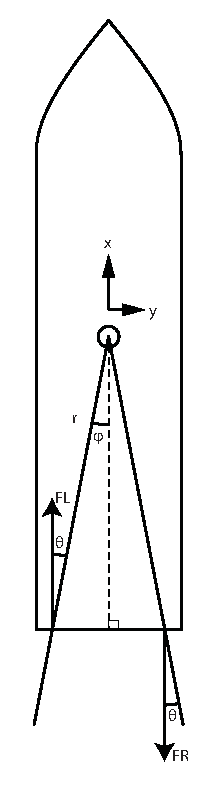
\includegraphics[angle=90]{img/boatmodel.pdf}[h]
\caption{By controlling FL and FR, it is possible to control the translational and rotational forces of the ship. The division of these forces is dependant on the angle of attack, $\theta$.}
\label{fig:forces}
\end{figure}
First we see that the boat is mirrored along it's X axis. From this we can set $\theta = \theta_L = \theta_R$ and $\phi = \phi_L = \phi_R$.  Now we have the forces, $F_L$ and $F_R$, as the controllable input to our system. These will be divided as into $F_X$, $F_Y$ and $\tau$, which are the variables that we wish to control. This division takes the form as seen in equation \eqref{Forceequation}.

\begin{equation}
\left[
\begin{matrix}
F_x\\
F_y\\
\tau
\end{matrix}
\right]
 =
 \left[
\begin{matrix}
\cos(\phi - \theta)\\
\sin(\phi - \theta)\\
\sin(\theta) \cdot r
\end{matrix}
\right]
\cdot F_R
+
 \left[
\begin{matrix}
\cos(\phi - \theta)\\
\sin(\phi - \theta)\\
-\sin(\theta) \cdot r
\end{matrix}
\right]
\cdot
F_L
\label{Forceequation}
\end{equation}
We observe that the motors will deliver force parallel to the x-axis, we can further set $\theta = \phi$. If this is the case $\sin(\theta - \phi)=0$, which nullifies the $F_Y$ term, and $\cos(\theta-\phi) = 1 \Longrightarrow F_X = F_L+F_R$ . The forces can then be modelled as equation \eqref{shortformforces}.
\begin{equation}
\left[\begin{matrix}
F_X\\
\tau
\end{matrix}
\right]
= 
\left[
\begin{matrix}
1\\
\sin(\theta)\cdot r
\end{matrix}
\right]
\cdot F_R
+ 
\left[
\begin{matrix}
1\\
-\sin(\theta)\cdot r
\end{matrix}
\right]
\cdot F_L
\label{shortformforces}
\end{equation}

\section{State Space form}
For better control of the system, it is desired to have the model of the ship in State Space form. This makes it possible to design an observer and a controller, which further makes it possible to design poles and zeros of the system.

The state space form for the system has the general form 
\begin{figure}[h]

\begin{equation}
\dot{x}=Ax+Bu
\end{equation}
\begin{equation}
y=Cx+Du
\end{equation}
\begin{tabbing}
Where \= $x$ is the state vector.\\
	\> $\dot{x}$ is the derivative of the state vector.\\
	\> $A$ is the state matrix\\
	\> $B$ is the input matrix\\
	\> $y$ is the output vector\\
	\> $C$ is the output matrix\\
	\> $D$ is the feedforward matrix
	
	
\end{tabbing}
\end{figure}

\chapter{Noise of measurements}
\label{ch:noise}
To facilitate a better estimate of the sensorvalues, the measurement noise is quantified and analysed, to allow for Kalman-filter to function as good as possible.

The noise can be generalized to the form
\begin{equation}
X(t) = Y(t) + W(t)
\end{equation}
\begin{tabbing}
Where \= X is the measured signal\\
	\> Y is the actual value\\
	\> W is the added noise 
\end{tabbing}
When considering measurements there will typically be two kinds of noise: Gaussian and Uniform. The uniformly distributed noise comes from the rounding error from discretizing the measurements, also known as quantization noise, while the normally distributed noise is present in the measurements themselves. This usually arises from the effect of background noise, imperfections in hardware, thermal noise, magnetic fields, as generated by the motors, and other sources. While some of these noise sources may have other distributions than the normal distribution, they are calculated as normal in accordance with the central limit theorem. The quantization noise is included in this assumption. From this assumption it is possible to describe the noise using only two parameters: The mean, $\mu$, and the variance, $sigma^{2}$.

\section{Inertial Measurement Unit}
The noise of the IMU is considering to be a zero mean process. From this it is easily seen that the variance of the noise can be estimated by letting the sensor be still and then logging the measurements. This process is documented in appendix \ref{chap:MeasJourIMU}. From this experiment the variance of the noise of the IMU measurements can be estimated as in table \ref{tab:IMUNoise}.

\begin{table}
\begin{tabular}{c|r l}
\textbf{Device} & $\boldsymbol\sigma ^2$ &\\
AccX & 5.05 & $\mu$G \\
AccY & 4.98 & $\mu$G \\
AccZ & 5.96 & $\mu$G \\
GyroX & 2.28 & $\frac{\mu ^\circ}{s}$\\
GyroY & 2.45 & $\frac{\mu ^\circ}{s}$\\
GyroZ & 2.40 & $\frac{\mu ^\circ}{s}$\\
MagX & & \\
MagY & & \\
MagZ & &\\
\end{tabular}
\end{table}
\label{tab:IMUNoise}
%\todo{Magnetometer variances}

\section{GPS}
The GPS is an important part of the system, as the validity of the depth measurements are very dependent on the GPS estimate at that particular time. Therefore a very precise noise variance estimation is important in order to calculate the actual position. The GPS works by precisely measuring the time signals sent from a number of satellites. These satellites are not stationary which means that the signal can wander from time to time. This is obvious in the measurements which were done, where the signal is wandering until it reaches a steady state. This could be estimated by including a bias in the model and estimating this. It has been decided not to implement such a feature for the moment. Instead the variance of the GPS measurements is calculated with this bias included, resulting in a larger variance.
According to the measurement journal, appendix \ref{chap:MeasJourGPS}, the variances are estimated to be 0.979 m and 1.12 m, for the $x$ and $y$ position, respectively.

\section{Velocity}
The estimate of the noise on the velocity measurements are assumed to be a zero-mean process with a given variance. The outputs of the measurements are however absolute values. This gives a different distribution of the measurements when the process is based around 0, than when it is distributed around another value. The distribution of the actual measurements is estimated to be shaped like the blue curve on fig \ref{fig:absdistrib}, while the underlying distribution is actual normal, like the red curve. If a normal distribution is fitted to the sampled data, the result is the green curve. Luckily the unbiased sample variance is defined as equation (\ref{eq:samplemean}), which means that the estimated sample variance is unconcerned with whether or not the samples are negative or absolute values.
\begin{equation}
s^2_{N-1} = \frac{1}{N-1} \sum^N_{i=1}(x_i-\overline{x})^2
\end{equation}
\label{eq:samplemean} For a zero mean process the sample variance is easily computed to be , as documented in appendix \ref{chap:MeasJourGPS}, to be $0.0026\frac{\mathrm{m}}{\mathrm{s}}$.
\begin{figure}[htbp]
	\centering
		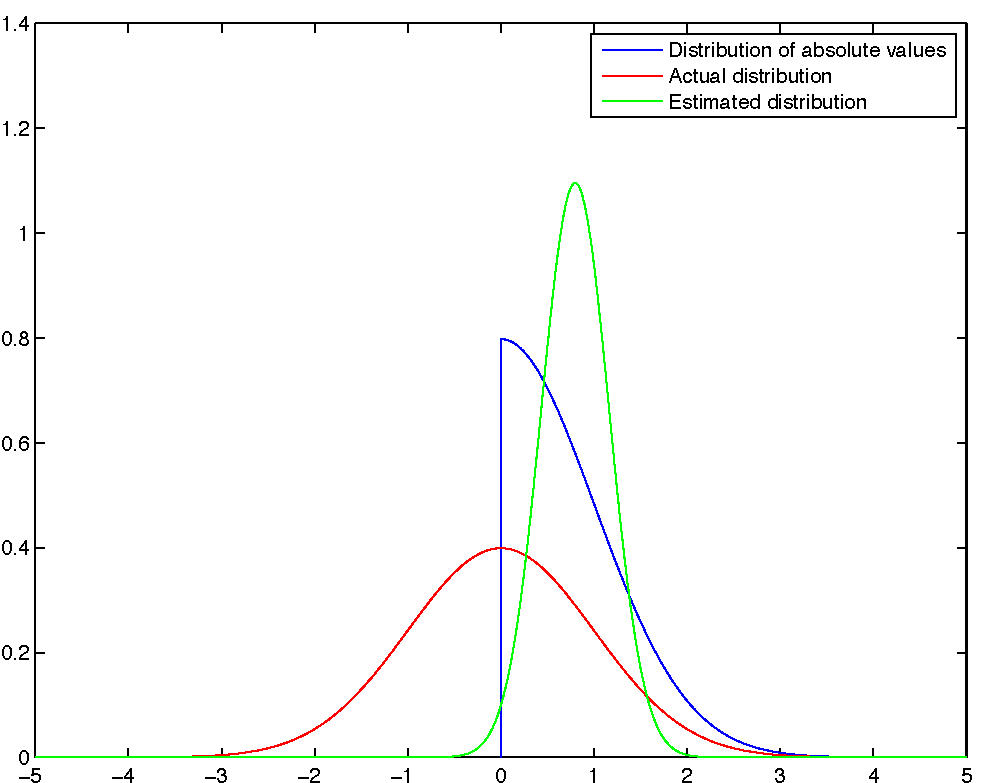
\includegraphics[width=\textwidth]{img/absdistrib.pdf}
	\caption{While the underlying distribution is normal (red), the absoluteness of the sampled data makes for a non-normal distribution (blue). If the variance and mean of the sampled data is taken, the result is the green curve.}
	\label{fig:absdistrib}
\end{figure}

\section{Position estimation}
To give a better position estimate which can be fed to the controller as well, the different data collected from the sensors mounted are put through a Kalman filter. This filter takes the different measurements as inputs, and uses these to give a better estimate of the position, rather than the quite noisy measurements taken using just the raw \ac{GPS} data. 

To develop such a filter, the model of the ship is to be computed, as well as a mapping of the different inputs and outputs to the system. The model of the forward and sidewards case (surge and sway) are quite easy to model, as these to are quite similar (the only difference being the drag coefficient being quite large for sideways motion). However, the heaving motion is complicated. 

\subsection{Surge and sway motion}
The state model for the surge and sway motion are quite similar, as the two consist of the same formula, but with different coefficients. The general formula for the position can be written as (in the discrete time domain):
\begin{align}
x(n+1) = x(n) + \dot{x}(n)t_s + \ddot{x}(n)\frac{t_s^2}{2}\\
\dot{x}(n+1) = \dot{x}(n) + \ddot{x}(n)t_s\\
\ddot{x}(n+1) = -\dot{x}(n) \cdot \overline{\alpha}_x(n) + \ddot{x}(n)
\end{align}
These formulae represent an estimate of the current position, velocity and acceleration given the previous measurements. As seen the above can be written in a matrix, to ease further computations:
\begin{align}
\begin{bmatrix}
x(n+1)\\
\dot{x}(n+1)\\
\ddot{x}(n+1)
\end{bmatrix} = \begin{bmatrix}
1 & t_s & \frac{t_s^2}{2}\\
0 & 1 & t_s\\
0 & -\overline{\alpha}_x(n) & 1
\end{bmatrix}\begin{bmatrix}
x(n)\\
\dot{x}(n)\\
\ddot{x}(n)
\end{bmatrix}
\label{eq:yn}
\end{align}
However, as the input to the system is given as an acceleration (the parameter that is controllable, given current inputs and measurements) - this can be taken out of the matrix, and inserted into an input vector:
\begin{align}
\vec{u}(n) = \begin{bmatrix}
0\\
0\\
\ddot{x}(n)
\end{bmatrix}
\label{eq:un}
\end{align}
The above equation \vref{eq:yn} combined with \vref{eq:un} describes the total motion forwards, which can be extended to the sideways case as well. To formulas are the same, the only thing that changes, is the drag coefficient. To model the drag coefficient, the drag coefficient can be estimated by:
\begin{align}
F_{drag} = \frac{1}{2}C_D \rho_w A_\text{hull} \dot{x} |\dot{x}|
\end{align}
\noindent Where:
\begin{ffk}
$C_D$ is a drag coefficient\\
$rho_w$ is the density of water\\
$A_hull$ is the cross-sectional area of the hull\\
\end{ffk}
This term is however nonlinear so to do further calculations on it, it would need to be linearized. The Taylor series expansion can be used. This is given as:
\begin{align}
f(x) \approx \overbrace{f(x_0) - \frac{\partial}{\partial x}f(x_0)\cdot x_0}^\text{constant} + \overbrace{\frac{\partial}{\partial x}f(x_0) \cdot x}^\text{variable}
\end{align}
The above represents a first order Taylor expansion and yields a constant and a variable term. The first order expansion of $F_drag$ gives the following expression:
\begin{align}
\overline{\alpha}_x(n) = \mathcal{T}(F_{drag} = \left(\frac{1}{2}C_D \rho_w A_\text{hull} \dot{x}_0^2 \dot{x}_0 - C_D \rho_w A_\text{hull} \dot{x}_0 \right) + (C_D \rho_w A_\text{hull} \dot{x}_0)\dot{x}
\end{align}

\subsection{Heave motion}
The heaving motion of the ship, will not immediatly take effect, as the ship will act as a "spring" when forced to move up, and will oscillate for a while, before it has reached its final position. To map this, a formula describing the forces given by \todo{indsæt kilde -rlc} is used. This formula describes the oscillation taking place when the ship is forced to move upwards. 
\begin{align}
\zeta = 2+2
\end{align}
\chapter{Software}

To implement the HLI functionality Python was chosen for its ease of writing as well as its extensive library of predefined functions. This enables the programmer to utilize highly complex functions through simple and  On of these libraries is NumPy, which enables the user to define vectors and matrices and do calculations with these, in the same way Matlab does. This made it easy to port Matlab code from simulation to actual implementation. Another library is the MatPlotLib library. This eased the path planning implementation, as it was possible to plot the result of the proposed algorithms during testing. Further, another Python library allowed the script to easily access the OpenStreetMap API and retrieve the relevant data.

The LLI functionality was implemented in C as this is the primary embedded programming language with which the project group has experience.

\section{System Description}

The HLI consists of 3 main modules and an additional simulator module, which is not rqeuired for the embedded application.

The main module of the software is the Ship Class and its function definitions.
The Ship Class itself represents an emph{actor} in the system. A Ship Object has individual dynamic model, controller and objective. Each Ship Object can plan its own waypoints, navigate trough them using their own sensor data and log informations.

\begin{center}
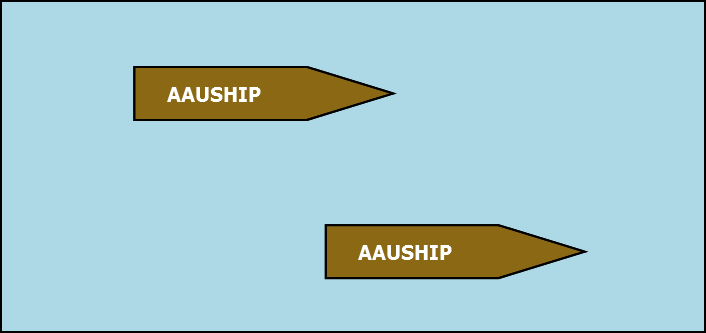
\includegraphics[width = 0.5\textwidth]{img/HLIFigures/ActorModel/Actor-model0.png}
\end{center}

A Ship Object requires auxillary Classes and Functions. The two side-modules of the system are the ObjectLibrary and FunctionLibrary. These Libraries store Classes and Functions, which are not directly connected to the physical behaviour of the ship, but provide an essential support for the Path Planning and Navigation control.

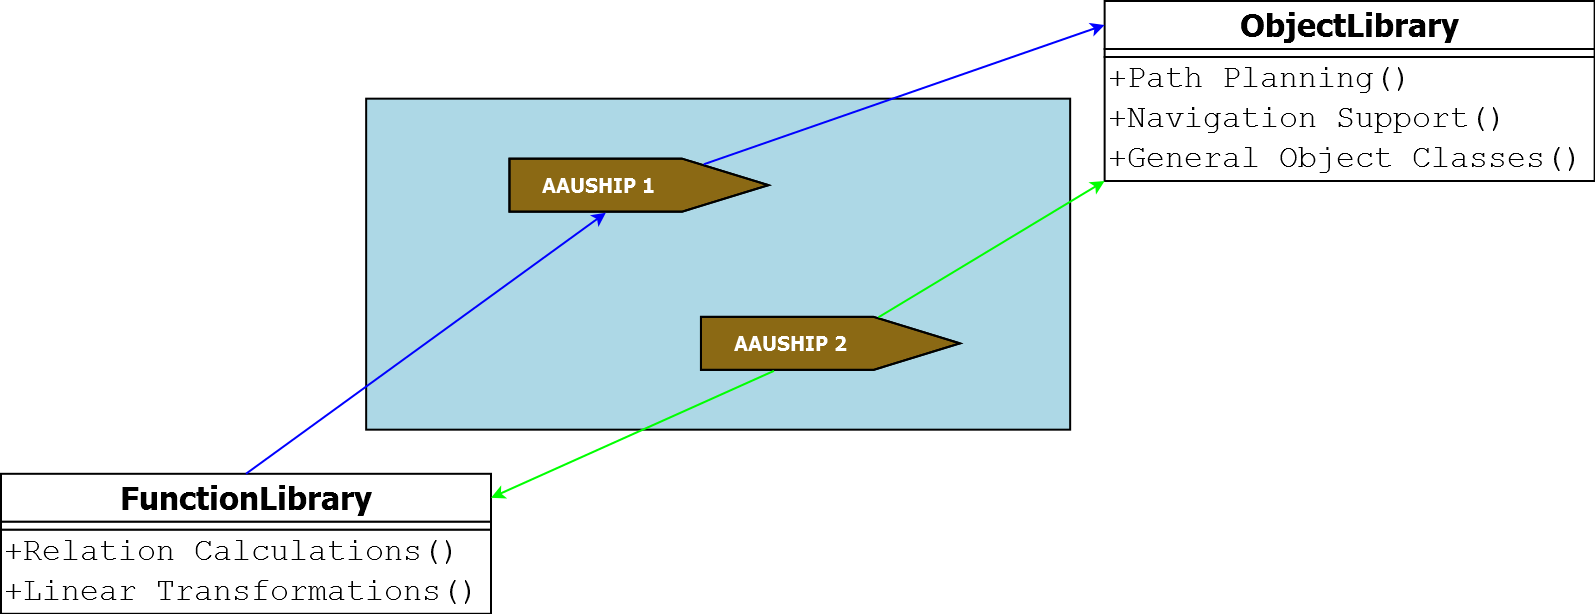
\includegraphics[width = \textwidth]{img/HLIFigures/ActorModel/Actor-model1.png}


Each ship calculates its own \emph{Waypoints}, depending on their individual capabilities and inputs.
There is a possibility for the ships to communicate trough a wireless channel with each other directly or trough a nearby mothership/computer, in order to share position data (to avoid collisions), or distribute the Path Planning tasks for enhanced computation power.

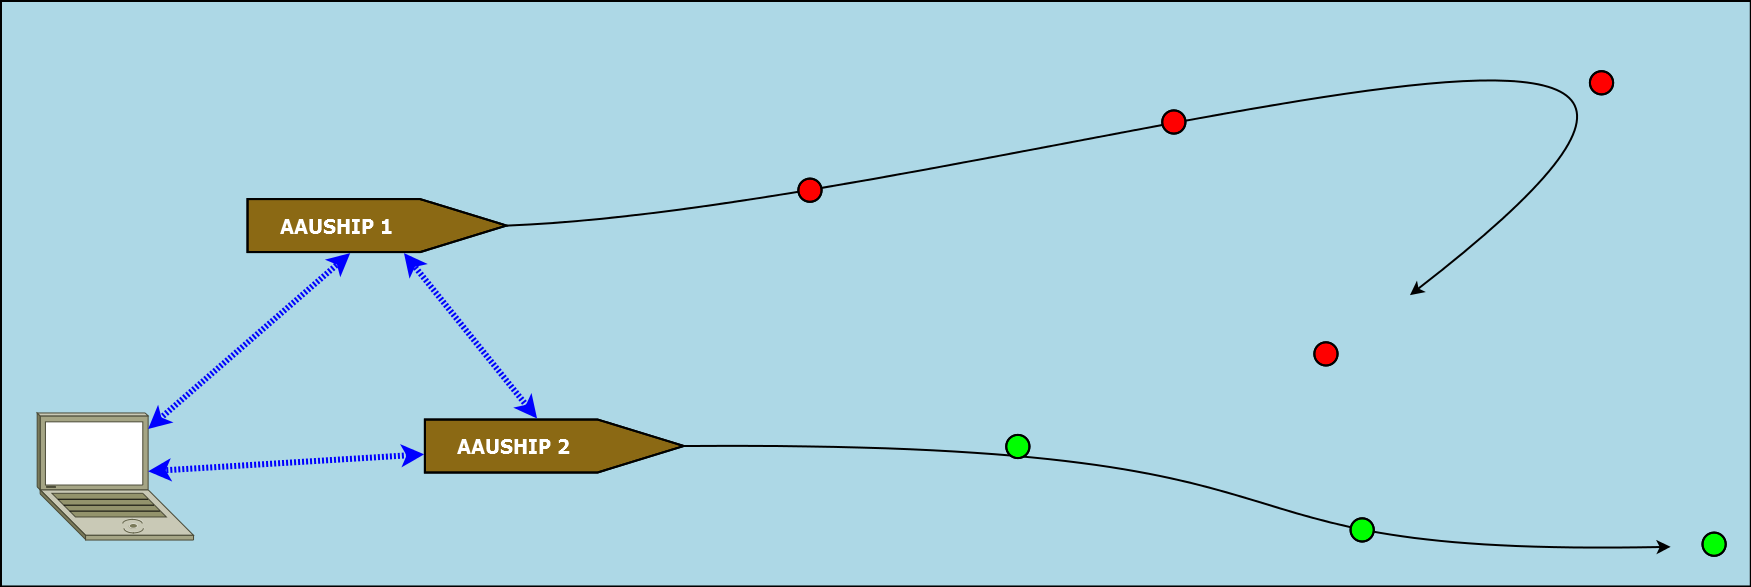
\includegraphics[width = \textwidth]{img/HLIFigures/ActorModel/Actor-model2.png}


The additional simulator module is an extension of the \emph{Ship Object}. In Simulation mode, to each \emph{Ship} belongs a \emph{Simulator}, simulating its interface communication and dynamic behaviour. The design of the simulator was led by two objectives:
\begin{itemize}
\item The \emph{Simulation} and the \emph{Embedded} application must run with the absolutely same \emph{Ship Class Module}
\item The simulator must predict the behaviour of the system well, but must be using a different model than the inner \emph{State Estimator Kalman Filter} of the ship
\item The simulator must be completely independent from the simulated system, except for the actuator values of the Ship.
\end{itemize}

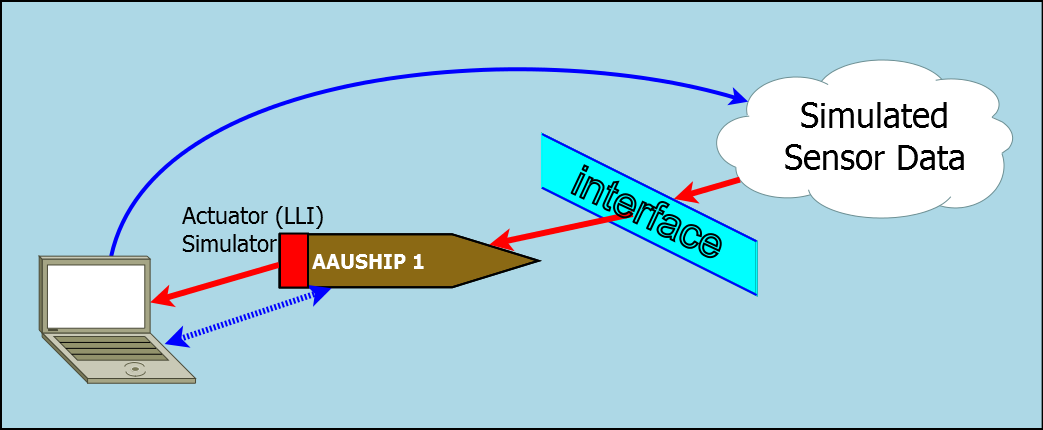
\includegraphics[width = \textwidth]{img/HLIFigures/ActorModel/SimModel.png}

Because of the predefined objectives above, the flowchart of the simulated and the actual task only slightly differs (Appendix)

%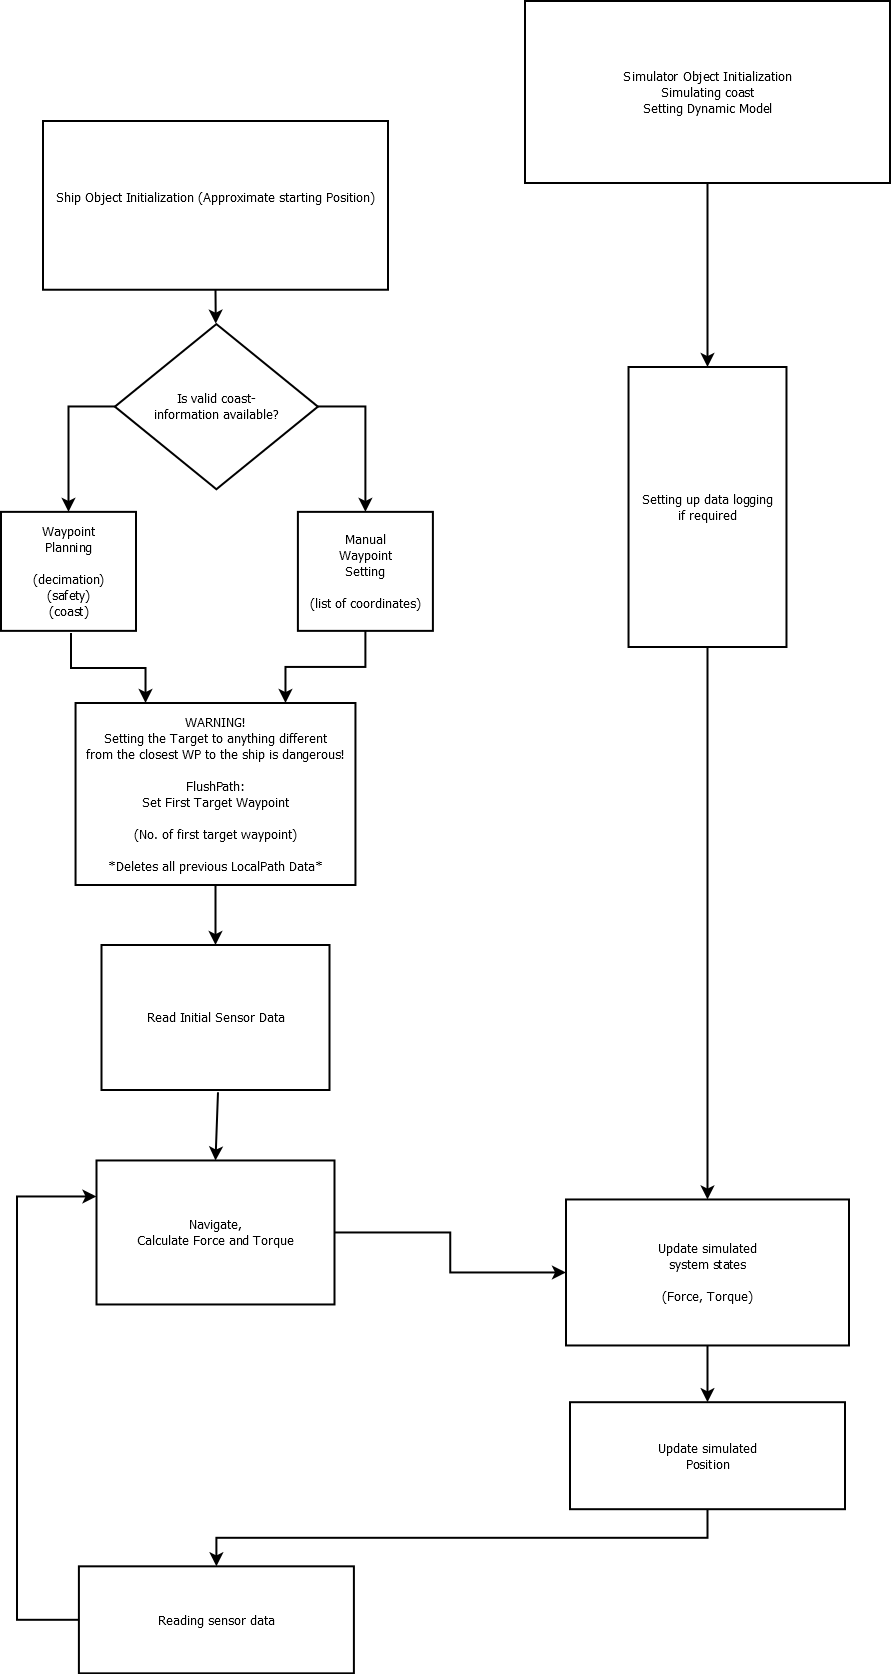
\includegraphics[width = \textwidth]{img/HLIFigures/System-Simulation_Interactions.png}

%The differences are kept on the right side of the Flowchart:

%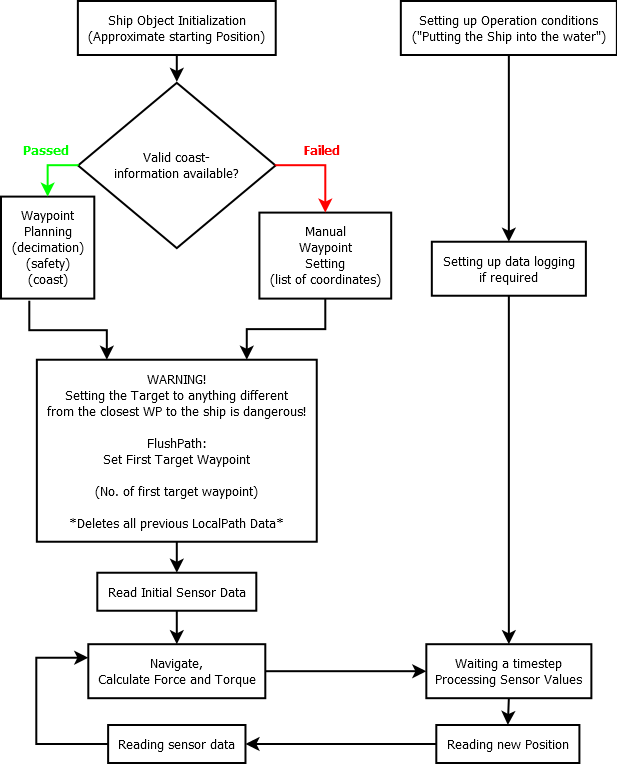
\includegraphics[width = \textwidth]{img/HLIFigures/System-World_Interactions.png}

\section{Course keeping control}

The Course-keeping control is responsible for keeping the ship on-course during Autonomous navigation.

The general idea is to have a state-space control algorithm in infinite loop as the main task. The control parameterization is based on the ship model, measurements and identification.
The program controls the ship along the specified path. If there is no next sub-\emph{Waypoint} or local path specified, the HLI calls the path planning methods for the next \emph{Waypoint}, then the procedure starts again from the beginning. If there are no more \emph{Waypoints}, the ship returns to the first \emph{Waypoint}, or to the starting coordinates specified in a subfunction of the Ship class.

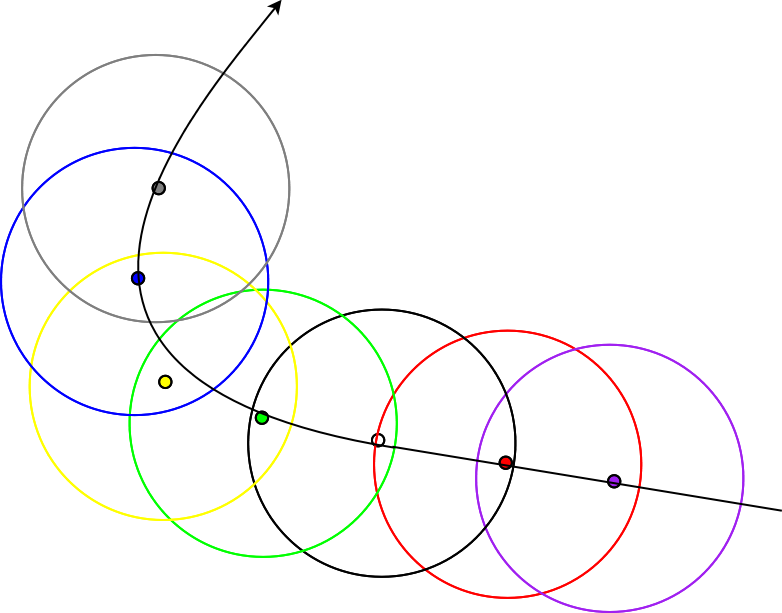
\includegraphics[width = \textwidth]{img/HLIFigures/SWPNavigationConcept.png}

Using Sub-\emph{Waypoints} instead of a full path line makes the navigation much easier. In open water there is significant sideways-motion caused by wind, ocean currents and waves, so staying perfectly true to a predefined path line is extremely difficult.
Instead, by using a series of Sub-\emph{Waypoints}, the navigation of the ship resembles to a series of Buoys guiding trough hazardous waters. The Ship approaches each Sub-\emph{Waypoint} in a predefined order and turns to the next, when the ''buoy´´ is close enough.
The characteristics of the navigation and course can be varied only by changing the definition of the Sub-\emph{Waypoints}, setting optimal parameters for different locations and settings.

\section{\emph{Waypoint} Planning}

The \emph{Waypoint}-planning system provides the basic routing for the autonomous navigation system.
The purpose of the \emph{Waypoint}-planning is to set key coordinates that the ship must approach, either for strictly defined reasons or to keep the ship away from forbidden or dangerous areas (like the coast or an island)

There are two possibilities to set a collection of \emph{Waypoints}: The operator can either manually set them, based on the GPS coordinates of the \emph{Waypoints}, or by inputting a coastline data series is a specified data type. The coast input format is a series of perpendicular distances measured from a line parallel to the coast. The coast input can be generated based on freely available map data (Openstreetmap).
The automatic \emph{Waypoint} planner divides the coast to smaller parts, based on the required oceanography definition. For each segment a minimum approach distance is calculated, and the \emph{Waypoint} planner defines a set of \emph{Waypoints} along the path in a snake way, or in any other predefined setting. The figure below shows a simulation of an oceanography task using automatic \emph{Waypoint} planning. All values in meters.
After the ship visited all of the \emph{Waypoints}, it returns to the first \emph{Waypoint}, or to a specified return position.

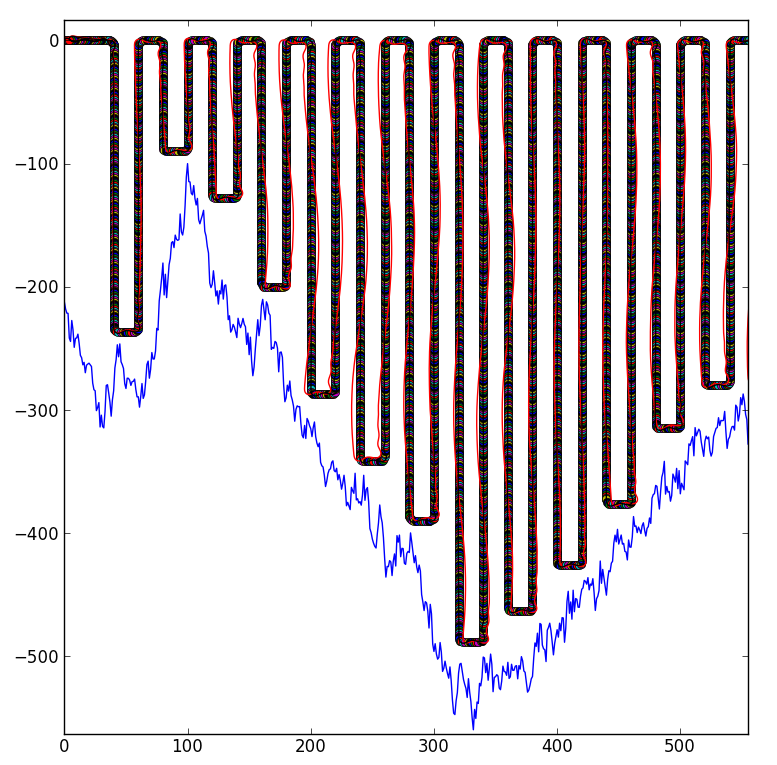
\includegraphics[width = \textwidth]{img/LocalPlannerFigures/Auto_WP_Planning.png}

Why are we using it?
The need for a basic \emph{Waypoint}-planner is essential, but optimizing it was not a high priority task. To test the prototype, a series of manually set \emph{Waypoints} are adequate.

\section{Local Planner}

The Local planner is responsible for planning a segment of the path, in order to supply the controller with a series of Sub-\emph{Waypoints}. The Local path should result in a set of points, which are lined up smoothly enough for the ship to sail through them with the reference speed.

The path can be divided to a straight line and a turning sub-path. The combination of a straight path and a turn is a Path Segment. The local planner calculates a Path Segment from the current position to the end of the turn at the next Turning \emph{Waypoint} (Footnote: If three \emph{Waypoints} are in a line, the angle at the second is $\pi$, therefore it is not a turning \emph{Waypoint}), based on the \emph{Waypoint} after the Turning \emph{Waypoint} as well.


\includegraphics[width = \textwidth]{img/LocalPlannerFigures/StraightRoute.png}

Calculating the smooth set of points for the turn:
The initial idea was to use a pre-generated Euler-spiral or simple arc line, the program determines the required arc length and applies linear transformations to resize and rotate the path coordinates, thus creating a smooth path.
The initial idea was dropped after the following considerations:
\begin{itemize}
\item Storing the full path coordinates is memory-consuming. Also, the path has either low resolution or the linear transformation would be CPU-heavy
\item The path would be smooth but would not have optimal parameters \ldots
\end{itemize}

The new idea is originated from: Koml\'osi Istv\'an: Mobilis robotok auton\'om navig\'aci\'oja mozg\'o akad\'alyok elker\"ul\'es\'evel (English version: Istv\'an Koml\'osi and B\'alint Kiss: Motion planning for multiple mobile robots using time-scaling).
The concept is to determine the maximum possible path curvature that the robot can handle. This is based on the Sigma and Kappa values of the Ship, where sigma is a function of the maximum speed of Torque change, and kappa is the maximum curvature of the path at a given speed. The local path is generated in a specific way that the robot will always turn with the maximum possible curvature at the current speed, thus staying the closest to the \emph{Waypoint} without losing speed. There is a threshold turn-angle, which determines if the robot requires only two identical Euler-spiral paths to turn or an arc path that has the maximum curvature, with two Euler spiral paths leading in or out.
In order to create the path the algorithm calculates 5 or 3 (depending on the threshold) key points and fits a Hermite-poly onto them. From this point on the local path in the given range is determined by these points only, thus saving memory and CPU time, while calculating a better path.
\begin{center}
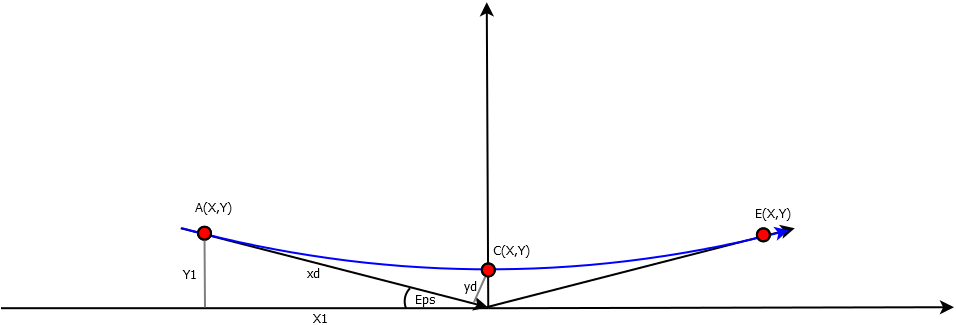
\includegraphics[width = \textwidth]{img/LocalPlannerFigures/3Points.png}
The calculation of the 3 key-points if $\epsilon < \epsilon_{max}$ (no circular path component is needed)

$$ \sigma = \frac{\beta_max}{v^2} $$
$$x_d = \frac{\pi}{\sigma} * C_F(\epsilon)$$
$$y_d = \frac{\pi}{\sigma} * S_F(\epsilon)$$

Where $C_F$ and $S_F$ are the normalized Fresnel-integral functions.

$$X_1 = x_d * cos(\epsilon) + y_d * sin(\epsilon)$$
$$Y_1 = X_1 * tan(\epsilon)$$

$$A = (-X_1, Y_1)$$
$$C = (0, \frac{y_d}{cos(\epsilon)})$$
$$E = (X_1, Y_1)$$

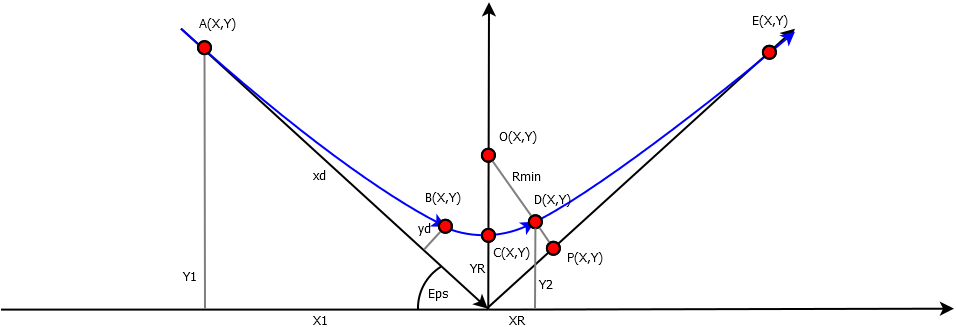
\includegraphics[width = \textwidth]{img/LocalPlannerFigures/5Points.png}
The calculation of the 5 key-points if $\epsilon > \epsilon_{max}$ (a circular path component is needed)

$$ \sigma = \frac{\beta_max}{v^2} $$
$$x_d = \frac{\pi}{\sigma} * C_F(\epsilon)$$
$$y_d = \frac{\pi}{\sigma} * S_F(\epsilon)$$

Where $C_F$ and $S_F$ are the normalized Fresnel-integral functions.

$$X_R = R_{min} * sin(\epsilon - \epsilon_{max})$$
$$P_X = X_R + y_d * sin(\epsilon)$$
$$X_1 = P_X + x_d * cos(\epsilon)$$
$$Y_1 = X_1 * tan(\epsilon)$$
$$P_y = Y_1 - x_d * sin(\epsilon)$$
$$Y_2 = P_y + y_d * cos(\epsilon)$$
$$O_Y = R_{min} * cos(\epsilon-\epsilon_{max) + Y_2}$$
$$R_Y = O_Y - R_{min}$$
$$X_2 = X_R$$

$$A = (-X_1, Y_1)$$
$$B = (-X_2, Y_2)$$
$$C = (0, Y_R)$$
$$D = (X_2, Y_2)$$
$$E = (X_1, Y_1)$$

\end{center}
The Hermite-polinom is used to populate the path with a number of points, depending on the predefined conditions. The resulting set of points is transformed to its correct place by a transformation matrix in the Local Frame, around the Turning \emph{Waypoint}.

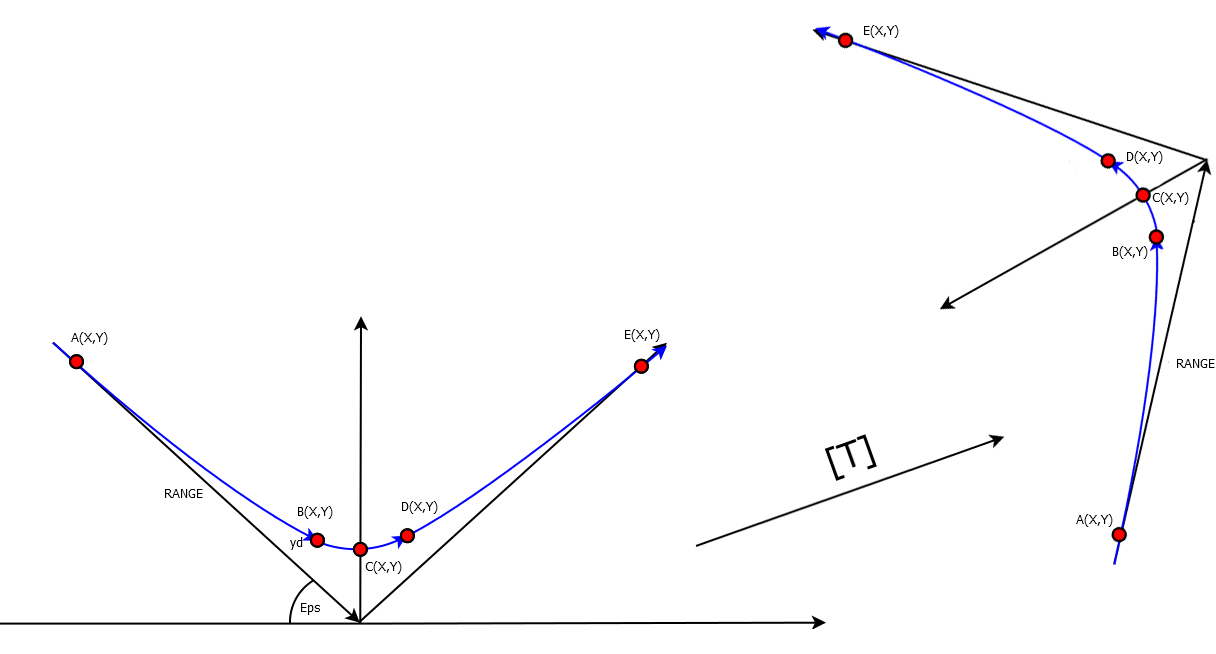
\includegraphics[width = \textwidth]{img/LocalPlannerFigures/PositioningTurn.png}

The considerations behind this path planning method were based on the following conditions:
\begin{itemize}
\item The ship must be able to output the next \emph{Waypoint} quickly, therefore calculating the whole path line in a single batch was to be avoided
\item The \emph{Waypoints} of the ship are subject to possible changes. Re-calculating the whole path every time a \emph{Waypoint} is changed is very consuming
\item The Ship is subject to unpredictable outside forces. Every path-segment is to be computed to be optimal, based on the actual, not the ideal prepared position
\item The local planning should be as efficient as possible. Planning every Sub-\emph{Waypoint} individually is a lot less effective than planning them in a batch \ldots
\end{itemize}

The Aurea mediocritas\footnote[1]{Golden mean} lies in dividing the path to segments, and planning the Sub-\emph{Waypoints} of each segment in a batch.


\chapter{Random notes about LLI concepts}
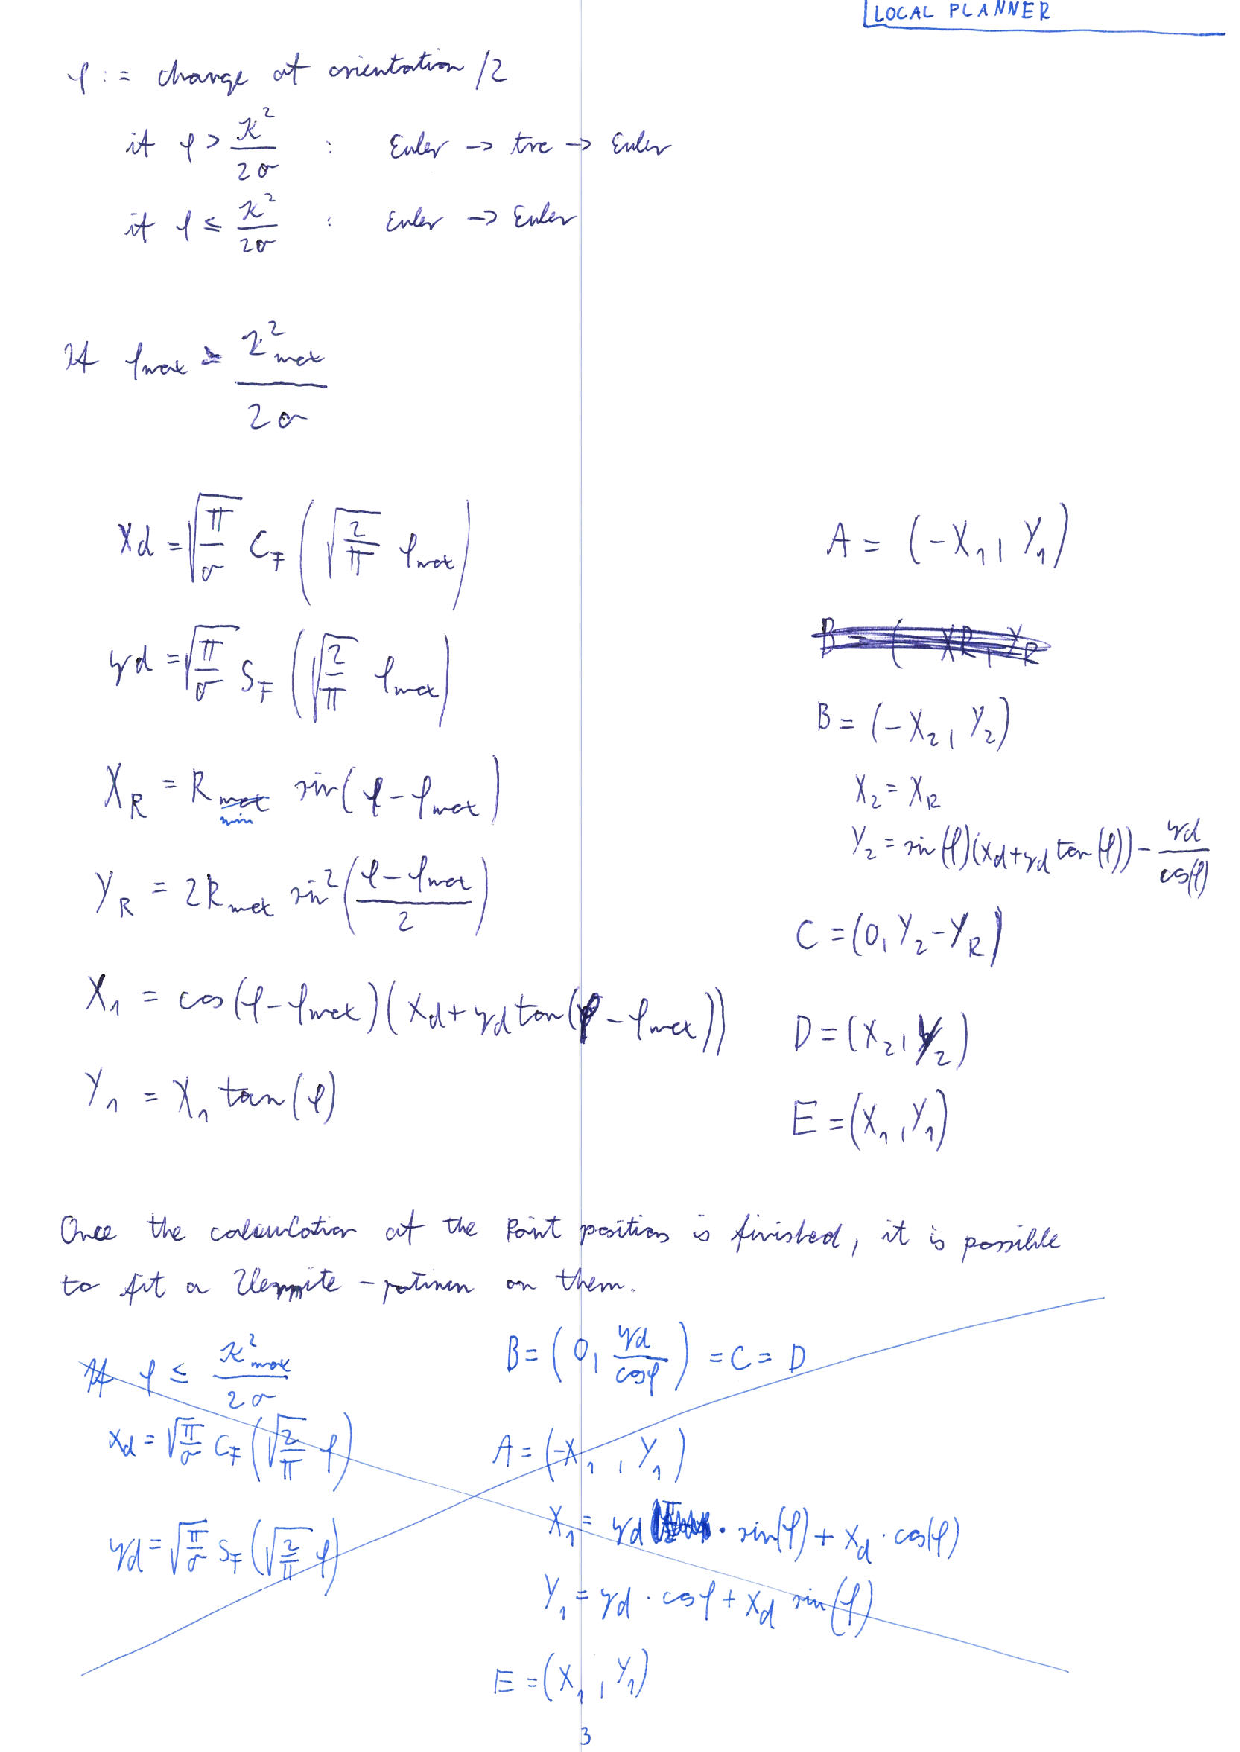
\includepdf[pages=-]{scans/hlinotes1}
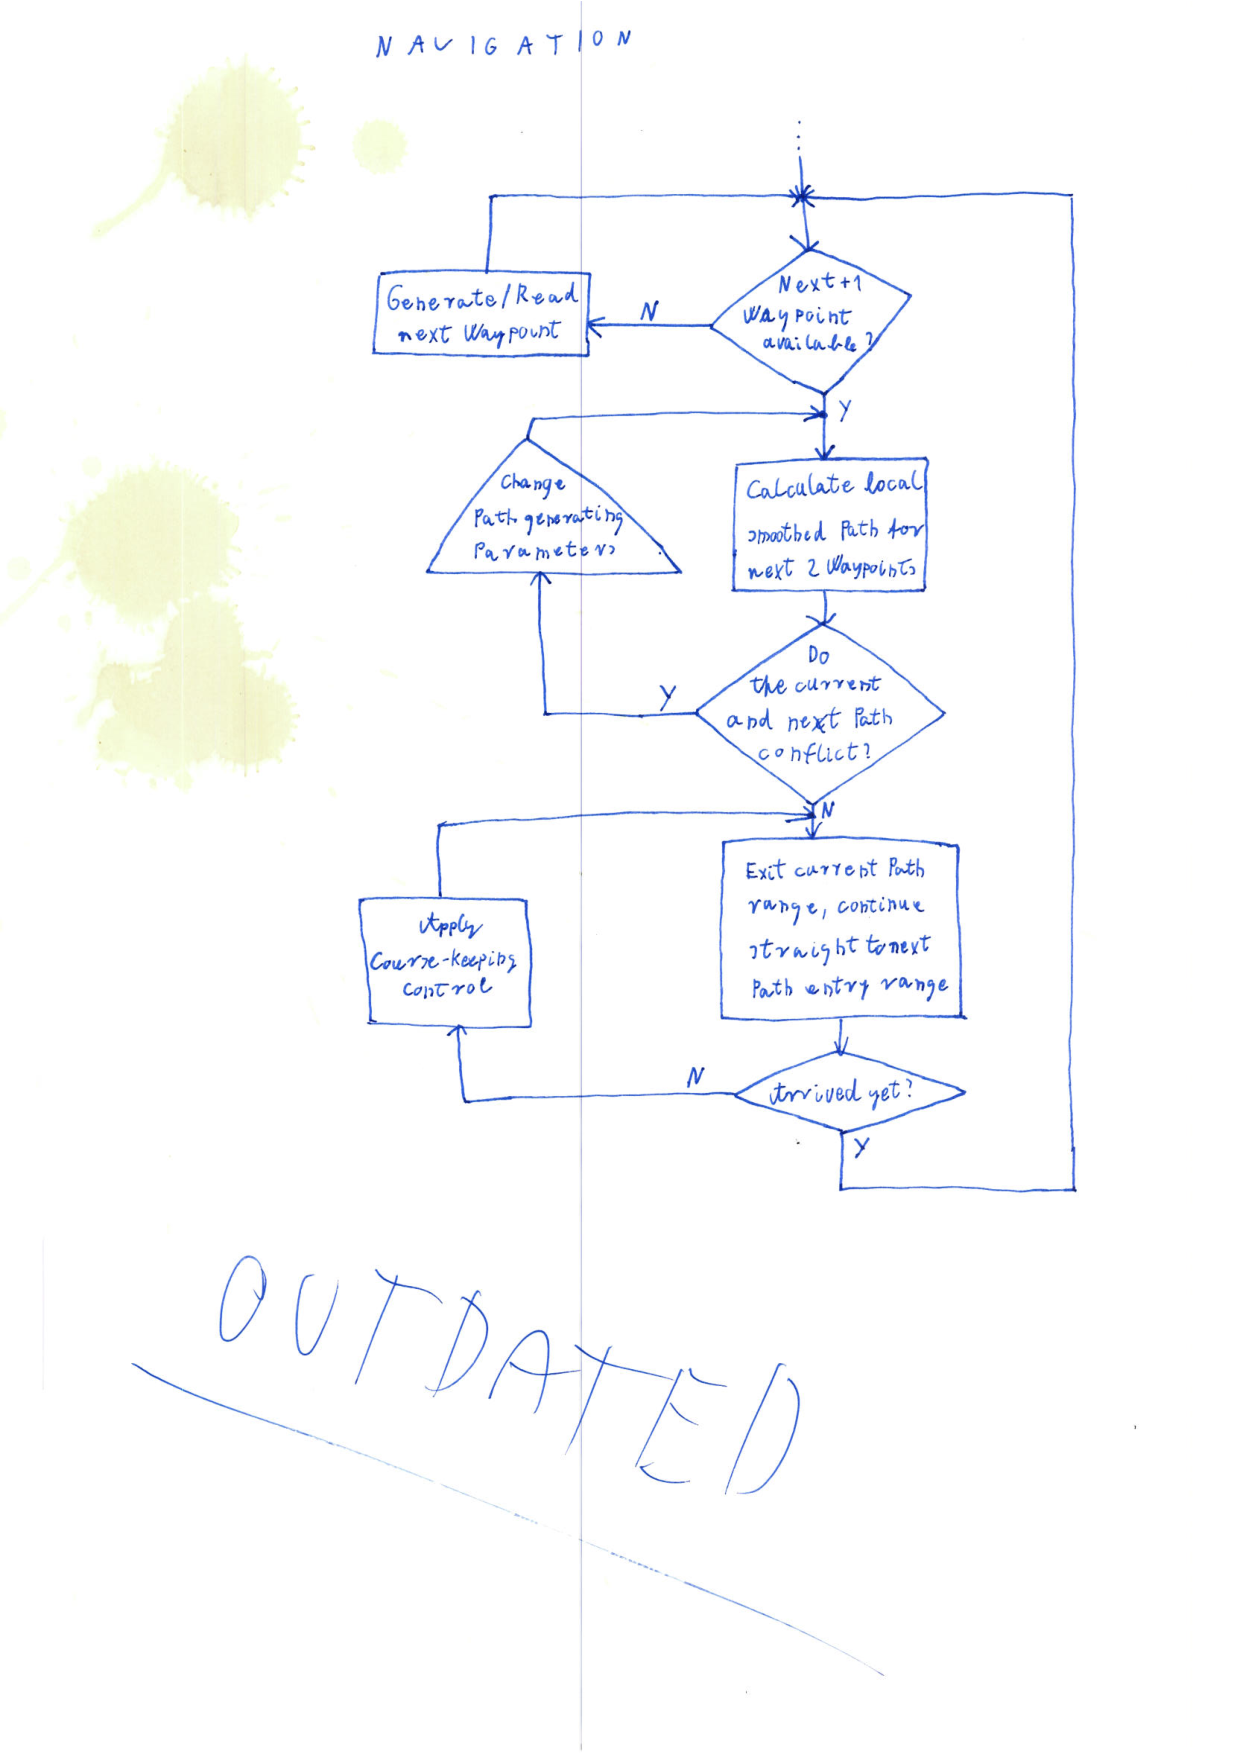
\includepdf[pages=-]{scans/hlinotes2}


\backmatter
\part{Appendices}
\appendix
\chapter{Measurement Journal: IMU Variance}
\label{chap:MeasJourIMU}
The intention of this journal is to measure the variance of the output of the ADIS16405 IMU.
\section{Equipment}
\begin{itemize}
\item ADIS16405
\item Macbook Pro 2010 15 inch 2.53 GhZ Intel Core i5, 4Gb Ram
\item APC220 Wireless communication Module
\end{itemize}

\section{Method}
A python script was implemented which logged the data which was accepted according to the protcol specifications chapter \ref{chap:Protocol}. The board on which the IMU is mounted is reading the data with a set delay between reads, and then bursting the data as soon as it has read. The data is timestamped when it is received by the python script. The script will keep running, receiving data, until it is cancelled. As it is very easy to gather samples, a large amount of samples has been gathered, by allowing the system to run overnight.\\
From an early trial run of the system it was discovered that the IMU would sporadically deliver measurements which were clearly wrong. Luckily all of the measurements were affected by this. Therefore it was possible to filter this by attaching the ADC of the IMU to ground, and then discarding the measurement when the ADC reads a high value.\\
The measurements are then input in Matlab and the variances of the measurements are estimated, using the 'var()' function.
\section{Measurements}
The measurements can be found in the file accdata.csv. The different values from the IMU are comma separated with each new measurement on a new line. The output follows the format: Voltage, X-,Y-,Z-Gyro, X-,Y-Z-Accelerometer,X-,Y-,Z-Magnetometer, Temperature, ADC.
\section{Results}
The resulting variance of the accelerometer measurements were found to be 5.05, 4.98, 5.96 $\mu$G for the X, Y and Z direction. 
For the Gyrometer the variances were found to be 2.28, 2.45 and 2.40 $\mu$degrees per second.
\chapter{Measurement Journal: GPS Variance}
The intention of this journal is to measure the variance of the output of the ADIS16405 IMU.\todo{change to GPS}
\section{Equipment}
\begin{itemize}
\item ADIS16405\todo{change to GPS}
\item \todo{brand and specs of computer (AAU registration number if possible)}
\item APC220 Wireless communication Module
\end{itemize}

\section{Method}
A python script was implemented which logged the data which was accepted according to the protcol specifications chapter \ref{chap:Protocol}. The board on which the IMU is mounted is reading the data with a set delay between reads, and then bursting the data as soon as it has read. The data is timestamped when it is received by the python script. The script will keep running, receiving data, until it is cancelled. The system was then set to run overnight.\\
It was expected to see the GPS wander for some time, but then to reach some form of steadystate where the measurements would primarily be affected by the measurement noise. This was clearly observed, as seen on figure \ref{fig:measgps} \\
\begin{figure}
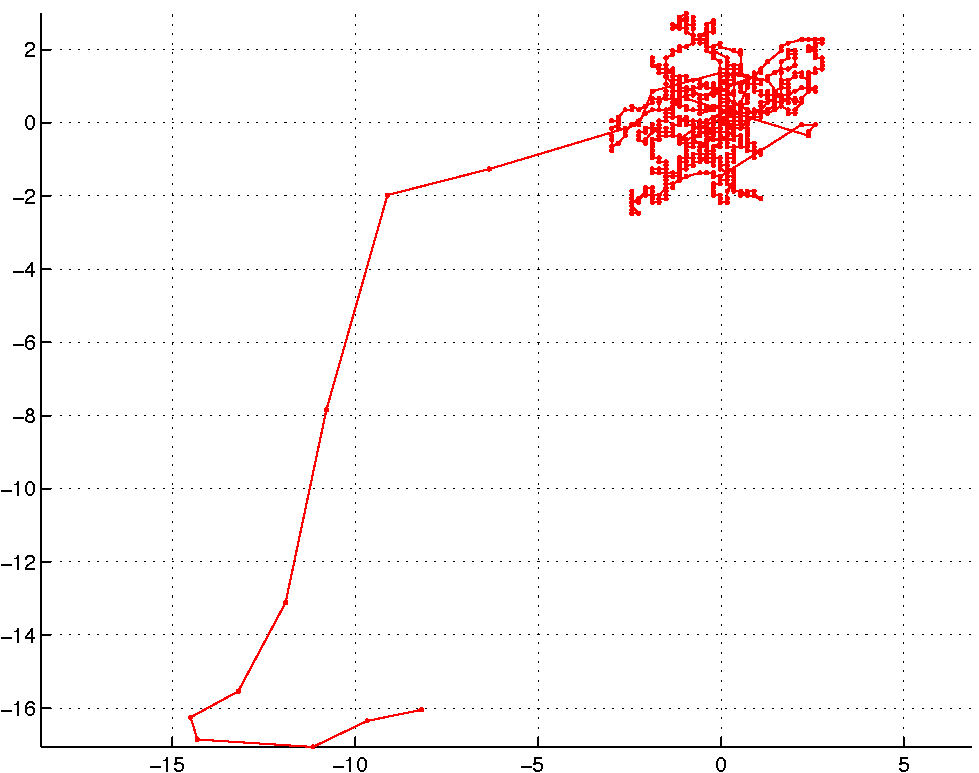
\includegraphics[width=\textwidth]{img/gpsmeas.pdf}
\caption{The GPS measurements, after being transformed into a local reference frame}
\end{figure}
\label{fig:measgps}

From an early trial run of the system it was discovered that the IMU would sporadically deliver measurements which were clearly wrong. Luckily all of the measurements were affected by this. Therefore it was possible to filter this by attaching the ADC of the IMU to ground, and then discarding the measurement when the ADC reads a high value.\\
The measurements are then input in Matlab, transformed into a local reference frame and the variances of the measurements are estimated, using the 'var()' function for the coordinate measurements. For the speed measurements, the unbiased sample variance formula as seen in equation (\ref{eq:measjournal:unbiassamplevariance}). Since the sample base is large, the effect of $\frac{1}{n}$ compared to $\frac{1}{n-1}$ is negligible, but the later should still be used, as the unbiased estimation is desired.

\begin{equation}
s^2_{N-1} = \frac{1}{N-1} \sum^N_{i=1}(x_i-\overline{x})^2
\end{equation}
\label{eq:measjournal:unbiassamplevariance}
\section{Measurements}
The measurements of the position can be found in gpsSDlog291112.log, while the speed data can be found in speedlog.log. As the speed measurements are not present in every sample from the GPS, the two files contain a different amount of samples. While position log contain 25220 measurements, the speedlog only contain 1690. This is however deemed sufficient for the variance estimate.
\section{Results}
The resulting variance of the GPS measurements were found to be 0.0026 $\frac{m}{s}$ for the speed measurements, while the variances for the position measurements were found to be 0.979 $m$ and 1.12 $m$, for the $x$ and $y$ position, respectively.
\chapter{Maiden Voyage}

After the boat had arrived and was properly equipped, everything was ready for a basic test with simple, manual control in order to observe its stability, its ability to take turns, as well as the speed the ship could navigate at. Because all pools or other forms of standing water were frozen at the time, this test had to be performed at the marina located \href{https://maps.google.com/?ll=57.058301,9.896772&spn=0.003495,0.009645&t=h&z=17""}{here}, on the corner of Skudehavnsvej and Vestre Fjordvej, in West Aalborg. 

\begin{figure}[htpb]
	\centering
	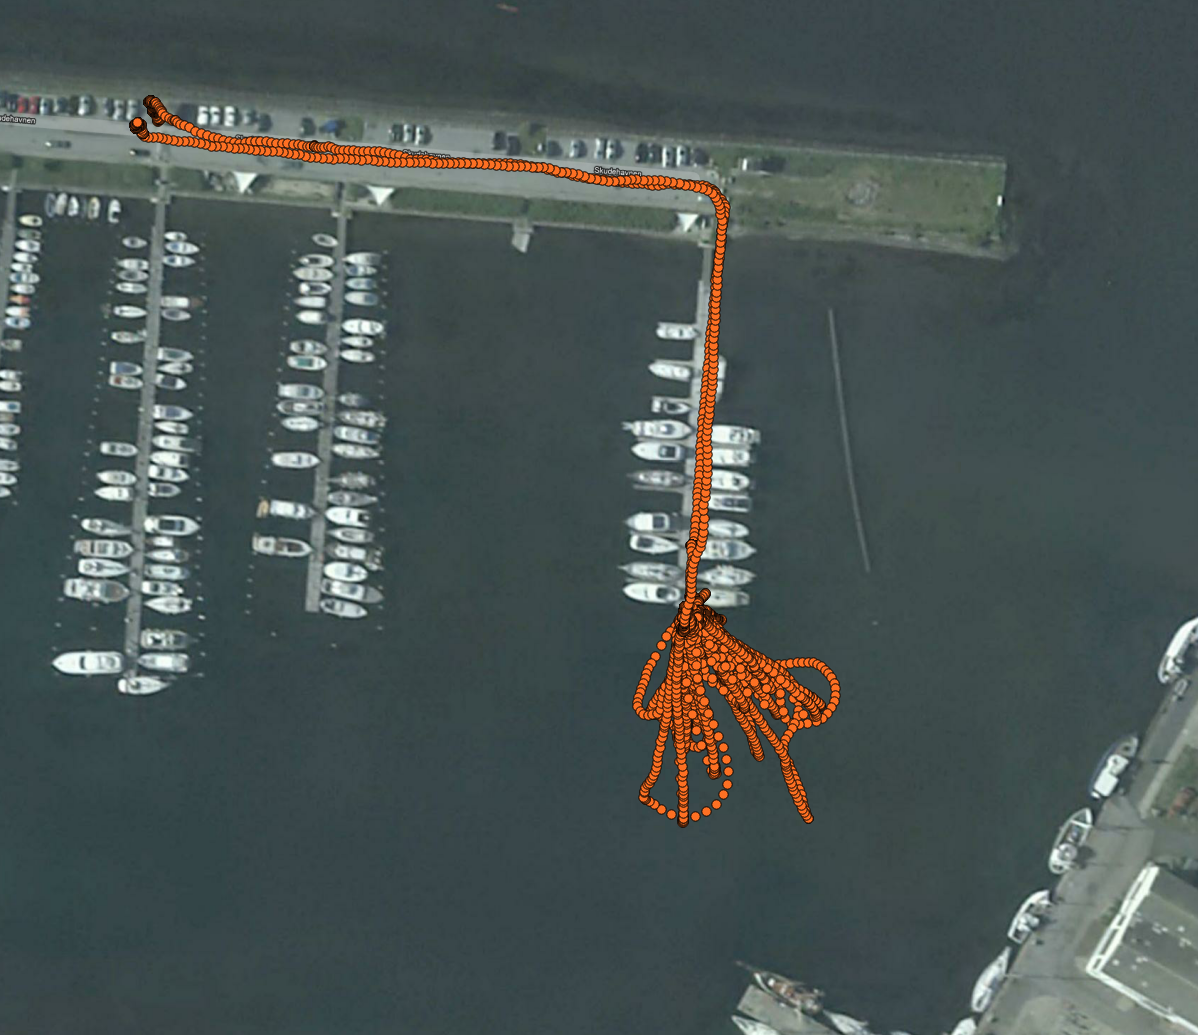
\includegraphics[width=\textwidth]{img/maidenVoyage/pointsOnMap}
	\caption{Manual control: GPS measurements with map} 
	\label{fig:pointsOnMap}
	\end{figure}

\begin{figure}[htpb]
	\centering
	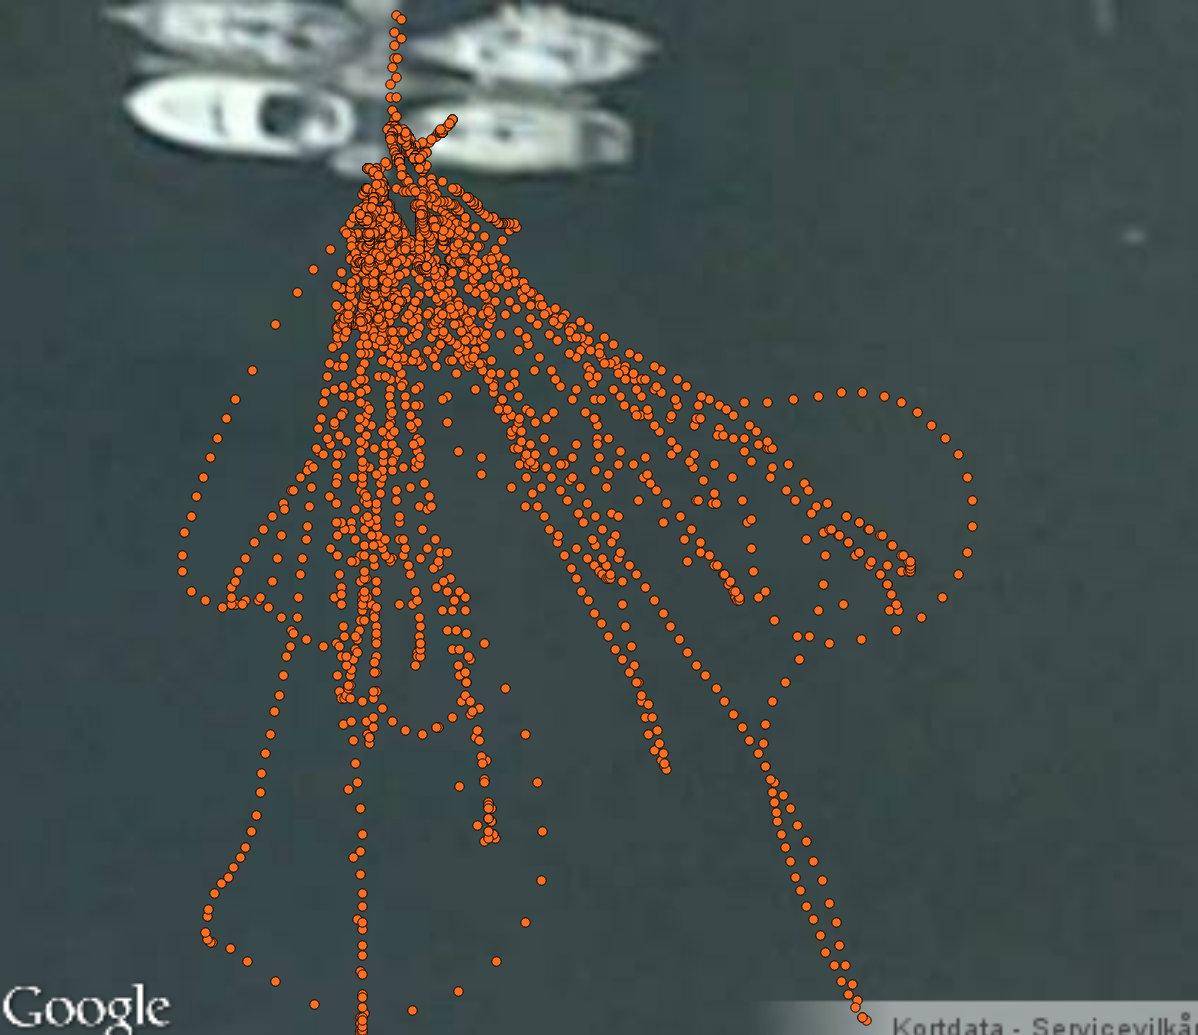
\includegraphics[width=\textwidth]{img/maidenVoyage/pointsOnMapZoom}
	\caption{Manual control: GPS measurements with map, zoom in} 
	\label{fig:pointsOnMap2}
\end{figure}

The boat was sealed with a lid and weighted with around 1.5 kg of lead in order to keep it as low in the water as possible, so that the propellers would not suck air in. Then a Python script was used which, when pressing "forward" or "back" would tell both motors to go faster of slower. The left arrow would increase the left propeller speed and would turn the right one down and vice versa. In this way, we were able to have basic control of the ship and test it. Space was used as an "emergency stop".

In pictures \vref{fig:pointsOnMap} and \vref{fig:pointsOnMap2} the data obtained from the GPS sensor during this trip is plotted on top of an Open Street map of the marina in which the tests took place. They begin in the top left of the picture, where we took the boat out of the car and walked to the water, then all the dots are the GPS messages received while performing sailing tests.

\begin{figure}[htpb]
	\centering
	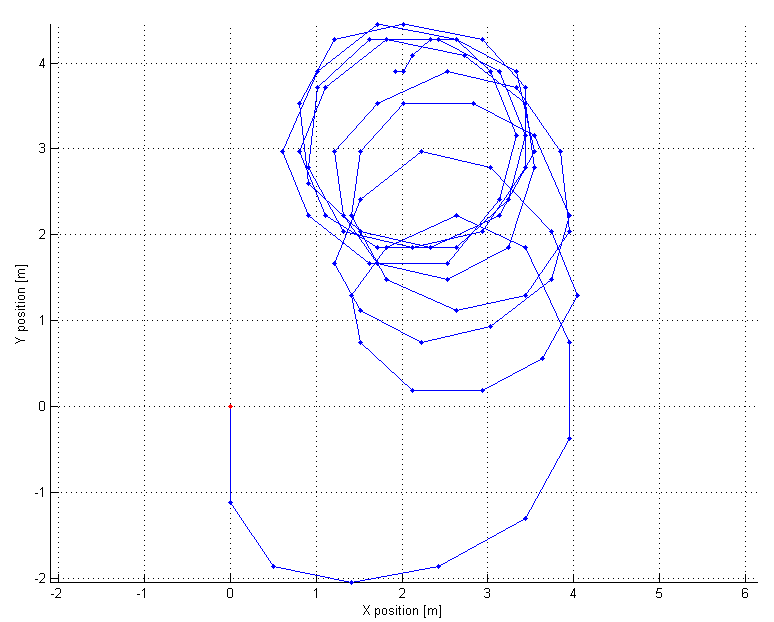
\includegraphics[width=\textwidth]{img/maidenVoyage/ship_turning2}
	\caption{GPS measurements of ship turning as logged by the LLI during maiden voyage} 
	\label{fig:ship_turning2}
\end{figure}

\begin{figure}[htpb]
	\centering
	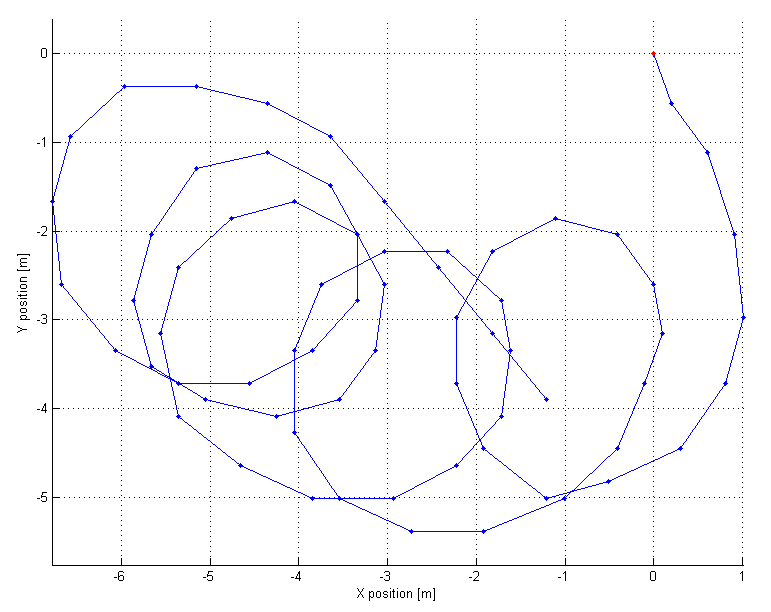
\includegraphics[width=\textwidth]{img/maidenVoyage/ship_turning}
	\caption{GPS measurements of ship turning as logged by the LLI during maiden voyage} 
	\label{fig:ship_turning}  
\end{figure}

Both Figure \vref{fig:ship_turning2} and \vref{fig:ship_turning} represent the ship in a continuous spiral. The turning radius will depend on the difference between the two motor speeds. It can be seen from the figures that this radius can be as small as 1 meter, which is a very good response. The red dot at (0, 0) represents the starting point.

The first wet test was also helpful in calibrating the control algorithm by noting that the motors are very powerful and that they should never be used at a very high throttle. Also, the motor controllers have some tolerance, meaning that the motors actually started turning forward at +10\% and reversing at -10\% of the available control signal. This hysteresis may induce jerks in the boat if not properly compensated because of overcompensating.




\chapter{Electronics schematics}
\label{chap:schema}
\head{This and the following pages is the schematics for the hardware developed.}

\todo{inset images of the finished products on thsi page}

\begin{figure}
\centering
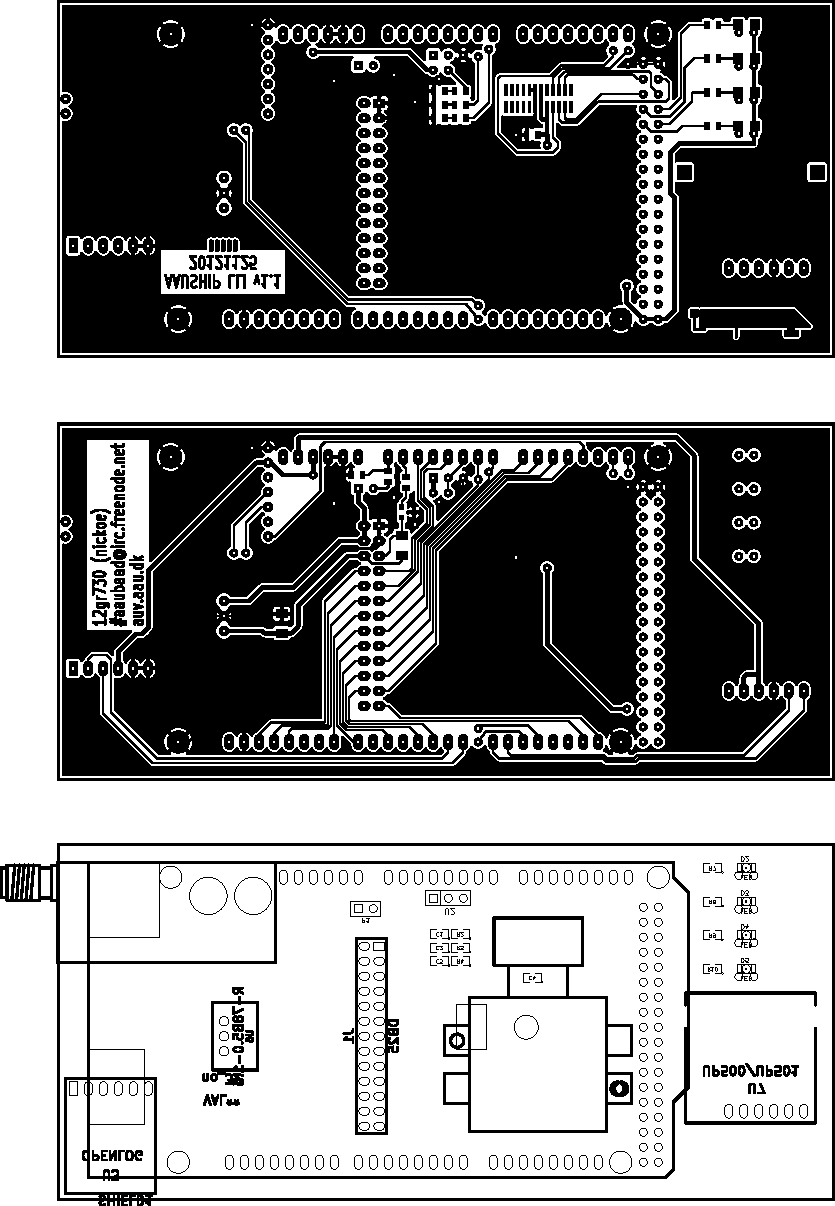
\includegraphics{img/lli-hw}
\caption{Hardware layout for the LLI}
\label{fig:lli-hw}
\end{figure}

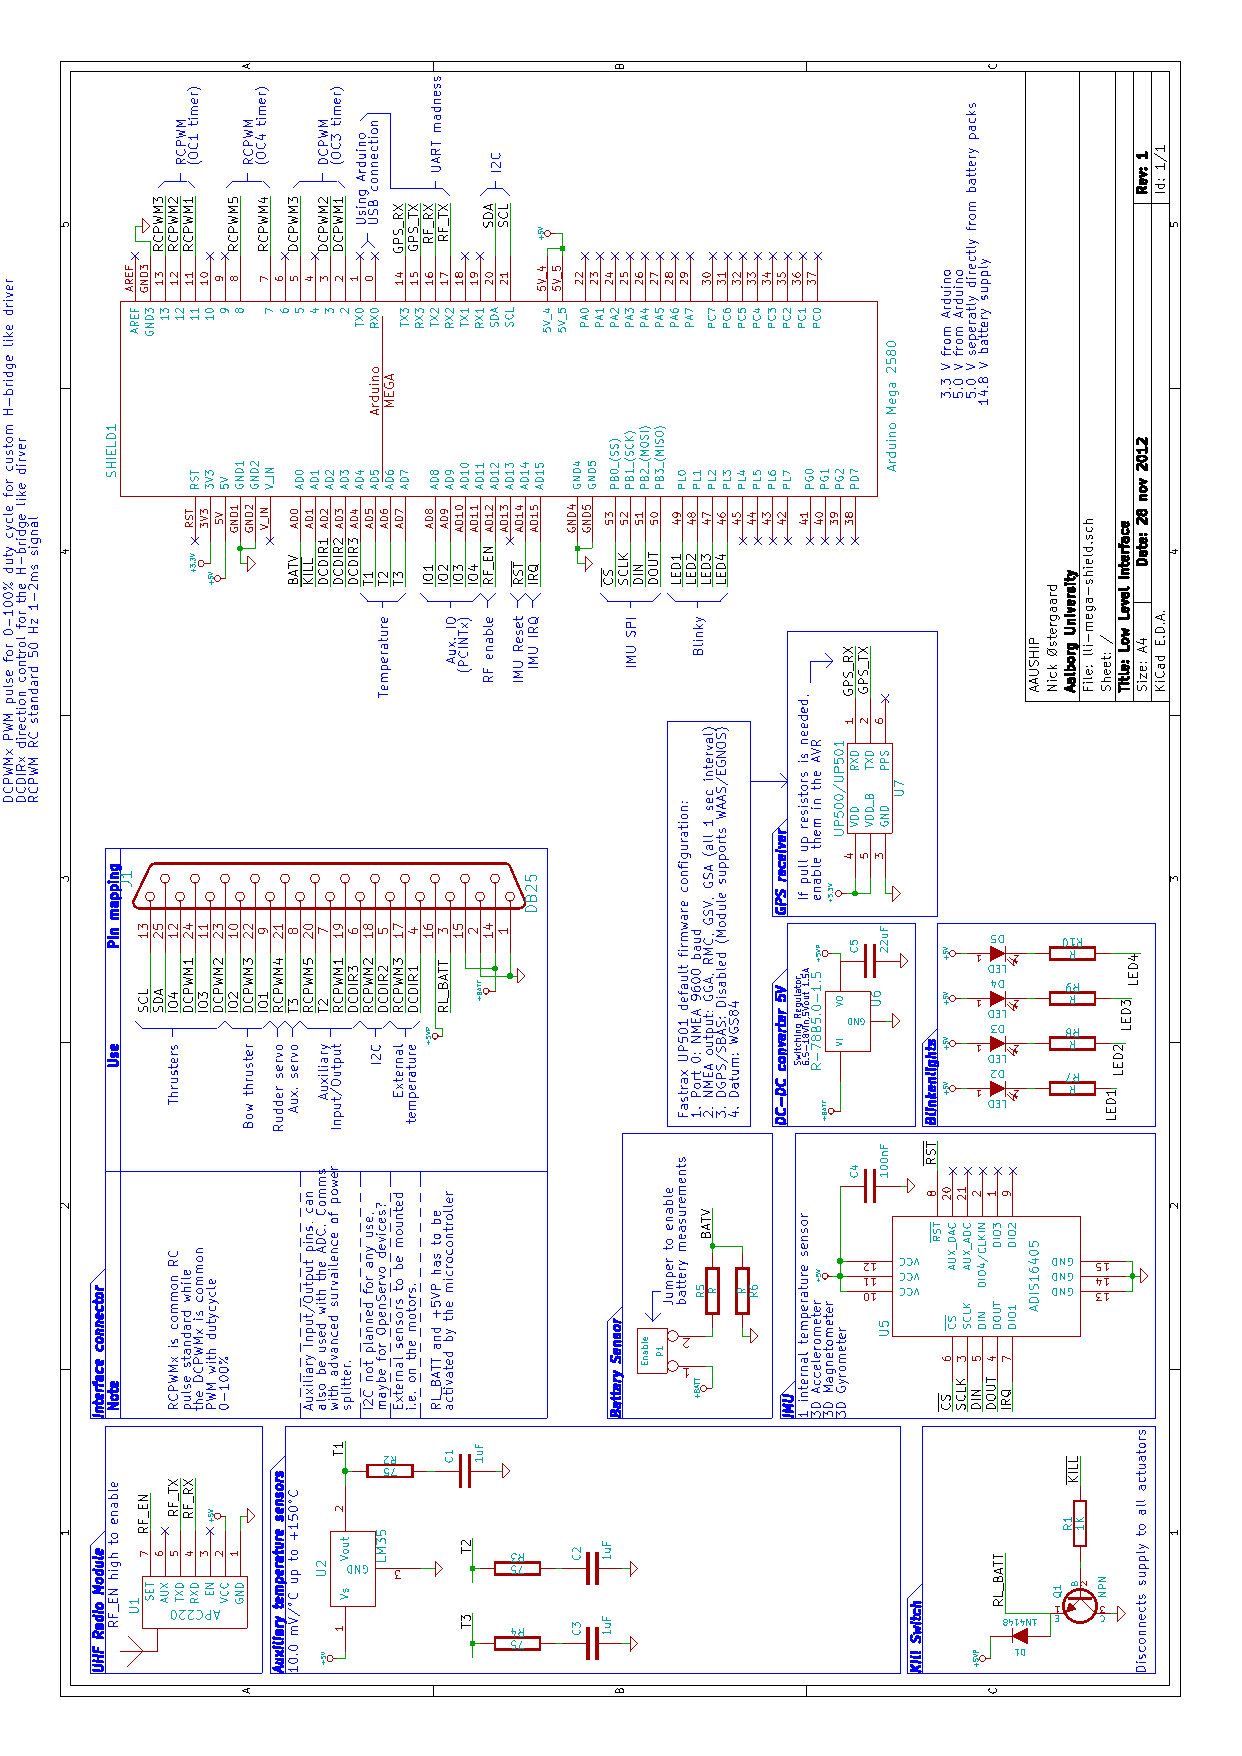
\includepdf{img/lli-mega-shield}
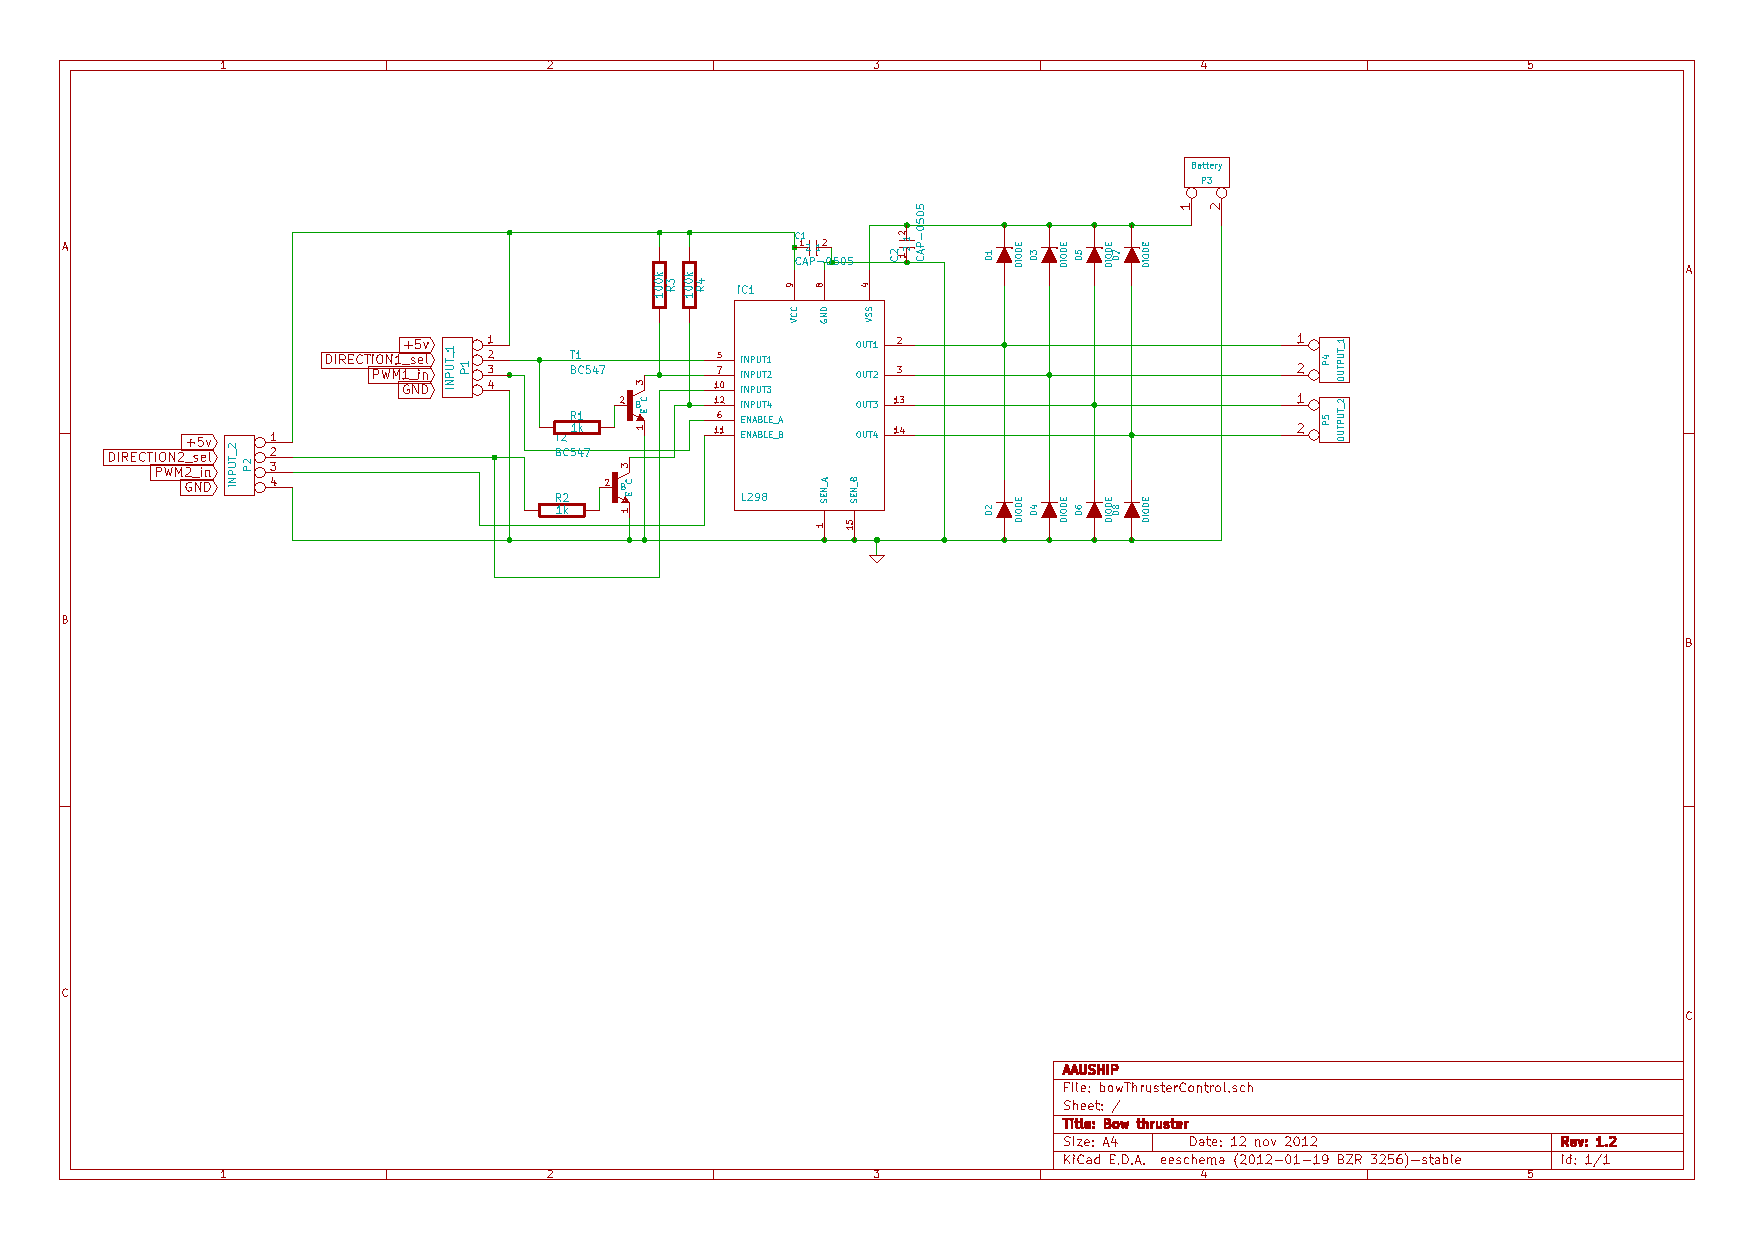
\includepdf{img/bow-thruster-schematic}
\label{appendices:bow thruster schematic}


\appendix
\chapter{System Flowcharts}
\label{chap:schema}
\head{The following Flowcharts demonstrate the slight difference between the simulated and embedded application.}

\begin{figure}
\centering

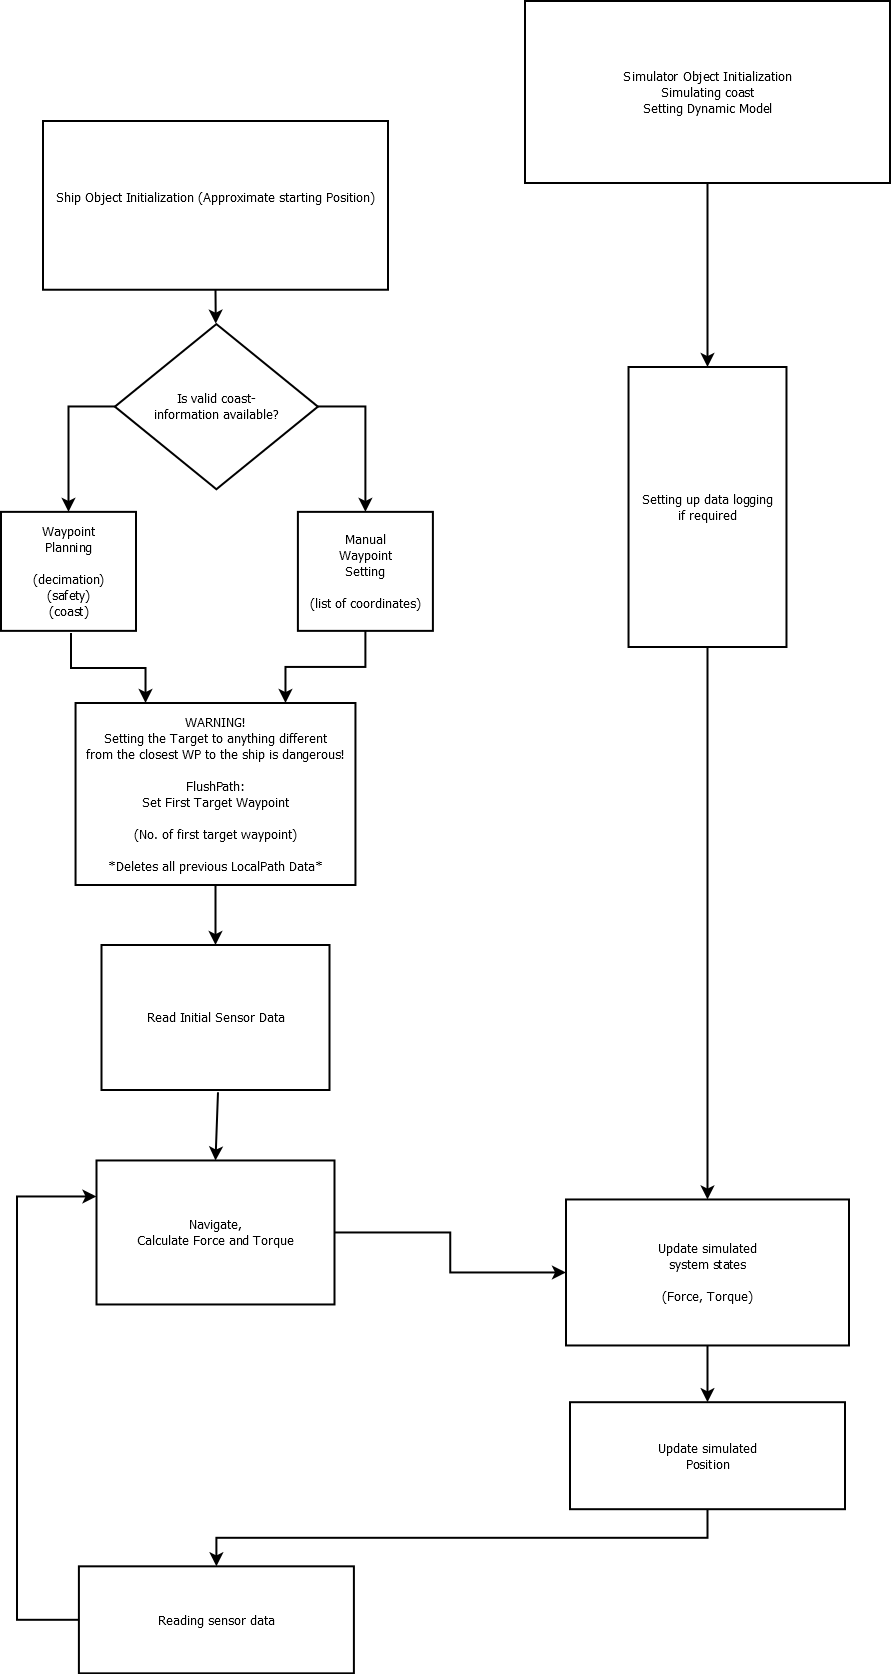
\includegraphics[width = \textwidth]{img/HLIFigures/System-Simulation_Interactions.png}
\caption{Flowchart of the Simulated Oceanography Task}
\label{fig:SimFlowchart}
\end{figure}

\begin{figure}
\centering
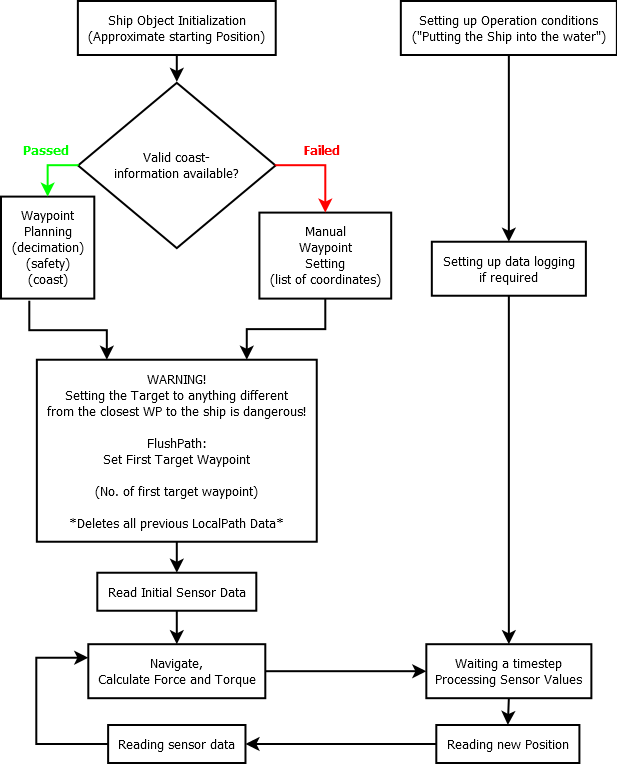
\includegraphics[width = \textwidth]{img/HLIFigures/System-World_Interactions.png}
\caption{Flowchart of the Embedded Oceanography Task}
\label{fig:EmbFlowchart}
\end{figure}



\bibliography{litterature}
\label{ch:litt}
\section{List of acronyms}
\begin{acronym}[TDMA]
  \acro{CRC}{Cyclic Redudancy Check}
  \acro{GPS}{Global Positioning System}
  \acro{GRS}{Ground Segment}
  \acro{HLI}{High Level Interface}
  \acro{IMU}{Inertial Measurement Unit}
  \acro{LLI}{Low Level Interface}
	\acro{OSM}{OpenStreetMap}
  \acro{SSS}{Single Screw Ship}
  \acro{SSM}{State Space Model}
  \acro{TSS}{Twin Screw Ship}
\end{acronym}



%\settocdepth{section}
\listoftodos
\end{document}

